\chapter{State of the Art} \label{State}

Nowadays, more and more computer-based scientific experiments need
to handle massive amounts of data. Their data processing
consists of multiple computational steps and dependencies within them.
A data-intensive scientific workflow (SWf) is useful
for modeling such process. Since the sequential execution of
data-intensive SWfs may take much time, 
Scientific Workflow Management Systems (SWfMSs)
should enable the parallel execution of data-intensive SWfs and exploit the resources distributed in different
infrastructures such as grid and cloud. 
This chapter provides a survey of data-intensive SWf management in SWfMSs and their parallelization techniques. This chapter is based on \cite{Liu2015}\cite{Liu2014a}.

Section \ref{sec:SOASWM} gives an overview of SWf management, including system architectures
and basic functionality. Section \ref{sec:SOAPES} focuses on the techniques 
used for parallel execution of SWfs. 
Then, Section \ref{sec:SOASMC} details the cloud computing including file system, multisite management in the cloud and the adaptation of SWfMSs to a multisite cloud environment.
Afterwards, Section \ref{sec:SOAOES} presents the recent frameworks for parallelization, eight SWfMSs and a science gateway to execute SWfs.
Finally, Section \ref{sec:SOACon} summarizes the main findings of this study and discusses the open issues raised for executing data-intensive SWfs in a multisite cloud. 

\section{Overview and Motivations}
\label{sec:SOAIntro}

Many large-scale scientific experiments take advantage of SWfs to model data operations such as loading input data, data
processing, data analysis, and aggregating output data. SWfs allow scientists to easily model and express the entire
data processing steps and their dependencies, typically as a directed
graph or Directed Acyclic Graph (DAG). As more and more data is consumed and produced in modern scientific experiments, SWfs become data-intensive. In order to process large-scale data within a reasonable time, they need to be executed with parallel processing techniques in the grid or the cloud. 

A SWf Management System (SWfMS)
is an efficient tool to execute workflows and manage data sets in
various computing environments. 
A SWfMS gateway framework is a system for SWfMS users to execute SWfs with different SWfMSs.
Several SWfMSs, \textit{e.g.} Pegasus \cite{Deelman2005,Deelman2014}, Swift \cite{Zhao2007},
Kepler \cite{Altintas2004}, Taverna \cite{Oinn2004}, Galaxy \cite{Goecks2010}, Chiron \cite{Ogasawara2013} and SWfMS gateway frameworks such as WS-PGRADE/gUSE \cite{Kacsuk2012} are now used intensively by various research communities, \textit{e.g.} astronomy,
biology, computational engineering. 
Although many SWfMSs exist, the architecture of SWfMSs have common features, in particular, the capability to produce a Workflow Execution Plan (WEP) from a
high-level workflow specification.
Most SWfMSs are composed of five layers, \textit{e.g.} presentation layer, user
services layer, WEP generation layer, WEP
execution layer and infrastructure layer. These five layers enable
SWfMSs users to design, execute and analyze data-intensive SWfs throughout the workflow lifecyle.

Since the sequential execution of
data-intensive SWfs may take much time, 
SWfMSs should enable the parallel execution of data-intensive SWfs and exploit large amounts of distributed resources.
Executable tasks can be generated based on diverse types of parallelism
and submitted to the execution environment according to different
scheduling approaches.

The ability to exploit large amounts of computing and storage
resources for SWf execution is provided by cluster, grid and
cloud computing.
Grid computing enables access to distributed, heterogeneous resources
using web services. These resources can be data sources (files,
databases, web sites, etc.), computing resources (multiprocessors, supercomputers,
clusters) and application resources (scientific applications, information management
services, etc.).
These resources are owned and managed by the institutions involved
in a virtual organization.

Cloud computing is the latest trend in distributed computing and has been the
subject of much hype. The vision encompasses on demand, reliable services provided
over the Internet (typically represented as a cloud) with easy access to virtually
infinite computing, storage and networking resources. Through very simple web
interfaces and at small incremental cost, users can outsource complex tasks, such
as data storage, system administration, or application deployment, to very large
data centers operated by cloud providers.
Since the resources are accessed through services, everything gets delivered as a
service. Thus, as in the services industry, this enables cloud providers to propose a
pay-as-you-go pricing model, whereby users only pay for the resources
they consume.
A  cloud is typically made of several sites (or data centers), each
with its own resources and data. Thus, in order to use more resources than
available at a single site or to access data at different sites, SWfs
could also be executed in a distributed manner at different sites.


There have been a few surveys of techniques for SWfMSs.
Some \cite{Bux2013} provide an overview of parallelization techniques for SWfMSs, including their implementation
in real systems, and discuss major improvements to the landscape of SWfMS.
Some other work \cite{Yu2005} examines the existing SWfMSs designed for
grid computing, and proposes taxonomies for different aspects of SWfMSs, including workflow design, information retrieval, 
workflow scheduling, fault tolerance and data movement.
In this chapter, we provide a survey of data-intensive SWf management in 
SWfMSs and their parallelization techniques and we focus on the following points:
\begin{enumerate}
\item A SWfMS functional architecture, which is useful to discuss the techniques for data-intensive SWfs.
This architecture can also be a baseline for other work and help with the assessment and comparison of SWfMSs.
\item A taxonomy of SWf parallelization techniques and SWf scheduling algorithms, and a comparative
analysis of the existing solutions.
\item A discussion of research issues for improving the execution of data-intensive SWfs in a multisite cloud.
\end{enumerate}


\section{Scientific Workflow Management }
\label{sec:SOASWM}

This section introduces SWf management, including
SWfs and systems. First, we define SWfs and SWfMSs. Then, we detail the functional
architecture and the corresponding functionality of SWfMSs. Finally,
we discuss the features and techniques for data-intensive SWfs
used in SWfMSs.


\subsection{Basic Concepts}

A SWfMS manages a SWf all along its life cycle. This
section introduces the concepts of SWfs, SWf life cycle, SWfMS and illustrates with SWf examples.


\subsubsection{Scientific Workflows}

A workflow is the automation of a process, during which data is processed
by different logical data processing activities according to a set
of rules. Workflows can be divided into business workflows and SWfs. Business workflows are widely used for business data processing.
According to the workflow management coalition, a business workflow
is the automation of a business process, in whole or part, during
which documents, information or tasks are passed from one participant
to another for action, according to a set of procedural rules \cite{Coalition1999}.
A business process is a set of one or more linked procedures or activities
that collectively realize a business objective or policy goal, normally
within the context of an organizational structure defining functional
roles and relationships \cite{Coalition1999}. Business workflows
make business processes more efficient and more reliable.

Different from business workflows, SWfs are typically
used for modeling and running scientific experiments. SWfs
can assemble scientific data processing activities and automate the
execution of these activities to reduce the makespan, which represents
the entire SWf execution time. A SWf is the assembly
of complex sets of scientific data processing activities with data
dependencies between them \cite{Deelman2009}. 
A SWf may contain one or several sub-workflows. A sub-workflow is composed of a subset of activities and data dependencies in the SWf while representing a step to process data.
SWfs can be represented in different ways. The most general representation
is a directed graph, in which nodes correspond to data processing
activities and edges represent the data dependencies.
But most often, a SWf is represented as a DAG or
even as a sequence (pipeline) of activities which is sufficient for
many applications.
Directed Cyclic Graphs (DCG) are harder to support since iteration is needed to represent repeated
activities, \textit{e.g.} with a whiledo construct \cite{Yu2005}.

Although business workflows and SWfs have some similarities,
they are quite different. 
The first difference is the abstraction level. Business workflows take advantage of traditional programming languages while SWfs exploit higher abstraction level tools to prove a scientific hypothesis \cite{Barker2007}. 
The second difference is the interaction
with participants. In business workflows, data can be processed by
different participants, which can be data processing machines or humans.
In SWfs, data is processed only by machines while
the scientists just need to monitor the workflow execution or control
execution when necessary. The interaction of humans during the execution of SWfs is much less than that of business workflows. 
The third
difference lies in the data flows and control flows \cite{Yildiz2009}.
Business workflows focus on procedural rules that generally represent
the control flows while SWfs highlight data flows
that are depicted by data dependencies \cite{Barker2007}. This is reasonable since scientific
experiments may need to deal with big experimental data. A data-intensive SWf processes, manages or produces
huge amounts of data during execution.
In addition, SWfs must be fully reproducible \cite{Barker2007}, which is not necessary for business workflows.

An activity is a description of a piece of work that forms a logical
step within a SWf representation. In a SWf, an activity defines the associated data formats and data
processing methods but requires associated data and computing resources
to carry out execution. The associated data in an activity consists
of input data and configurable parameters. When the configurable parameters
are fixed and the input data is provided, the execution of a workflow
activity is represented by several tasks. A task is the representation
of an activity within a one-time execution of this activity, which
processes a data chunk. An activity can
correspond to a set of tasks for different parts of input data. Sometimes,
\textquotedblleft{}jobs\textquotedblright{} are used to represent the meaning of tasks \cite{Bux2013} or activities \cite{Chen2012a,Deelman2014}.



\subsubsection{Scientific Workflow Life Cycle}
\label{sec:subsub:SWLC}

The life cycle of a SWf is a description of the state
transitions of a SWf from creation to completion
\cite{Deelman2009,Gorlach2011}. A SWf life
cycle generally contains four phases. G\"{o}rlach \textit{et al.} \cite{Gorlach2011}
propose that a SWf life cycle contains modeling phase,
deployment phase, execution and monitoring phase, and analysis phase.
Deelman \textit{et al.} \cite{Deelman2009} argue that a SWf life cycle consists of composition phase, mapping phase,
execution phase and provenance phase. 
Provenance data represents information regarding workflow execution \cite{Freire2008}.
We present provenance in more details in the next section. 
In \cite{Mattoso2010}, a provenance database is proposed to represent and relate data from several phases of the workflow life cycle.
In this chapter, we adopt a combination of workflow life cycle views \cite{Deelman2009,Gorlach2011,Mattoso2010} with a few variations, condensed in four phases:
\begin{enumerate}
\item The composition phase \cite{Deelman2009,Mattoso2010} is for the creation of an abstract SWf.
An abstract SWf is defined by the functionality of each activity (or sub-workflow) and data dependencies
between activities (or sub-workflows) \cite{Gottdank2014,Tersty2014}. 
SWf composition can be done through a textual or Graphical User Interface (GUI). 
SWfMS users can reuse the existing SWfs with or without modification \cite{Holl2012}.
\item The deployment phase \cite{Gorlach2011} is for constructing a concrete SWf, 
which consists of concrete methods (and associated codes) for each functional activity (or sub-workflow) defined in the composition phase, so that the SWf can be executed. 
\item The execution phase \cite{Deelman2009,Mattoso2010} is for the execution of SWfs with associated
data, during which input data is processed and output data is produced.
\item The analysis phase \cite{Gorlach2011,Mattoso2010} is to apply the output data to scientific experiments, to analyze SWf provenance data and to share the SWf information.
\end{enumerate}

\subsubsection{Scientific Workflow Management Systems}

A Workflow Management System (WfMS) is a system that defines, creates,
and manages the execution of workflows. A WfMS is able to interpret
the workflow process definition typically in the context of business applications.
A SWfMS is a WfMS that handles and manages SWf execution. 
It is powerful tool to execute SWfs in a SWf
engine, which is a software service that provides
the runtime environment for SWf execution \cite{Balasko2014}.
In order to execute a SWf in a given environment,
a SWfMS typically generates a Workflow Execution Plan (WEP), which is a program that captures optimization decisions
and execution directives, typically the result of compiling and optimizing a workflow, before execution. 

To support SWf analysis, SWfMS should support additional functionality such as provenance. 
SWf provenance may be as (or more) important as the scientific
experiment itself \cite{Freire2008}.
Provenance is the metadata that captures the derivation history of a dataset, including the original data sources, intermediate datasets, and the SWf computational steps that were applied to produce this dataset \cite{Costa2013,Oliveira2012a,A.R.Gonccalves2012,Horta2012}.
Provenance data is used for SWf analysis and SWf reproducibility.

\subsubsection{Scientific Workflow Examples}
\label{subsubsec:SWE}

SWfs have been used in various scientific domains.
In the astronomy domain, Montage%
\footnote{Montage project: http://montage.ipac.caltech.edu/%
} is a computing and data-intensive application that can be modeled
as a SWf initially defined for the Pegasus SWfMS. This
application is the result of a national virtual observatory project
that stitches tiles of images of the sky from diverse sky surveys
into a photorealistic single image \cite{Deelman2008}. Montage is
able to handle a wide range of astronomical image data
including the Two Micron All Sky Survey, (2MASS%
\footnote{2MASS: http://www.ipac.caltech.edu/2mass/%
}), the Digitized Palomar Observatory Sky Survey, (DPOSS%
\footnote{DPOSS: http://www.astro.caltech.edu/\textasciitilde{}george/dposs/%
}), and the Sloan Digital Sky Survey (SDSS%
\footnote{SDSS: http://www.sdss.org/%
}) \cite{Jacob2009}. Each survey possesses huge amounts of data and
covers a corresponding part of sky in visible wavelengths or near-infrared
wavelengths. 2MASS has roughly 10 terabytes, DPOSS has roughly 3 terabytes
and SDSS contains roughly 7.4 terabytes. All the data can be downloaded
from a corresponding server at the aforementioned links and then
staged into the execution environment, such
as a shared-disk file system or a database, in order to be processed.

\begin{figure}
\centering{}
\captionsetup{justification=centering}
\includegraphics[width=84mm]{figures/1}\caption{\textbf{The structure of a small Montage workflow \cite{Singh2008}. }}
\label{fig:Sf1} 
\end{figure}

The structure of a small Montage workflow (at task level) is shown in Figure \ref{fig:Sf1}, where each node represents a task.
The number within a node represents the name of a task in the SWf. The tasks at the same line represent one activity.
The first activity (Tasks $1-6$) has no parent activities. Each of them exploits an mProject program to project a single image to the scale defined in a pseudo-FITS header template file. The second activity (Tasks $7-14$) utilizes an mDiffFit program to create a table of image-to-image difference parameters. The third activity (Task $15$) takes advantage of an mFitplane program to fit the images generated by former activities ($7-14$) to an image. 
The fourth activity (Task $16$) uses an mBgModel program to interactively determine a set of corrections to apply to each image to achieve a \textquotedblleft{}best\textquotedblright{} global fit according to the image-to-image difference parameter table. The fifth activity (Tasks $17-22$) removes a background from a single image through an mBackground program. 
The sixth activity (Task $23$) employs an mImgtbl program to extract the FITS header information (information about one or more scientific coordinate systems that are overlaid on the image itself) from a set of files and to create an ASCII image metadata table. Finally, the seventh activity (Task $24$) pieces together the projected images using the uniform FITS header template and the information from the same metadata table generated by Task $23$. This activity applies an mAdd program. 

\begin{figure}
\centering{}
\captionsetup{justification=centering}
\includegraphics[width=129mm]{figures/f2}\caption{\textbf{SciEvol workflow \cite{Ocana2012}. }}
\label{fig:Sf2} 
\end{figure}

In the bioinformatics domain, SciEvol \cite{Ocana2012} is a SWf
for molecular evolution reconstruction that aims at inferring evolutionary
relationships on genomic data. To be executed in the Chiron SWfMS, SciEvol consists of 12 activities as shown in Figure \ref{fig:Sf2}. The first activity (pre-processing FASTA file) is a Python script to format
the multi-fasta input file.
FASTA file is a textual presenting format for nucleotide
or peptide sequences. 
The second activity (MSA construction) constructs
a Multiple Sequence Alignment (MSA) using a MAFFT program (or other
MSA programs). A MAFFT program is generally for generating the alignment of three or more biological sequences (protein or nucleic acids) of similar length. 
The third activity (MSA conversion) executes ReadSeq to convert the MSA
in FASTA format to that in PHYLIP format, which is used in the phylogenetic tree construction activity. 
The fourth activity (pre-processing PHYLIP file) formats the input file (referenced as \textquotedblleft{}phylip-file-one\textquotedblright{}) according to the format definition and generates a second file (referenced as \textquotedblleft{}phylip-file-two\textquotedblright{}).
The fifth activity (tree construction) receives the \textquotedblleft{}phylip-file-one\textquotedblright{}
as input and produces a phylogenetic tree \cite{Felsenstein1989} as output. 
The sixth activities (evolutionary analysis from $6.1$ to
$6.6$) analyze the phylogenetic tree with corresponding parameters and
generate a set of files containing evolutionary information as
output. 
Each of the activities (evolutionary phases) is related to one of
six codon substitution models, which are used to verify if the
groups of genes are under positive Darwinian selection.
These activities exploit the same program using different parameters.
The last activity (data analysis) automatically processes
the output files obtained from the previous activities. 

There are many other data-intensive SWfs in bioinformatics. For
instance, SciPhylomics \cite{Oliveira2013} is designed for producing
phylogenomic trees based on an input set of protein sequences of genomes
to infer evolutionary relationships among living organisms. SciPPGx
\cite{Dias2012} is a computing and data-intensive pharmacophylogenomic
analysis SWf for providing thorough inferring support for pharmacophylogenomic
hypotheses. SciPhy \cite{Ocana2011} is used to construct phylogenetic
trees from a set of drug target enzymes found in protozoan
genomes. All these bioinformatics SWfs have been executed using
SciCumulus SWfMS \cite{Oliveira2010}.

The components of SWfs can be classified by their
functionality, motifs, or structure patterns. The functionality can be
data processing, activity scheduling, activity execution, and resource
management \cite{Altintas2004}. The motifs may be data-oriented and
workflow-oriented. Data-oriented motifs consist of recurring activities
such as data storage \cite{Balasko2014}, data analysis, data cleaning,
data moving \cite{Balasko2014} and data
visualization. Workflow-oriented motifs may correspond to remote
invocations, repetitive activities, parameter sweep workflows and meta-workflows \cite{Balasko2014,Garijo2014}.
A parameter sweep workflow is a workflow with multiple input parameter sets, which needs to be executed for each input parameter set \cite{Chirigati2012,Gottdank2014}. 
A meta-workflow is a workflow composed of sub-workflows. 
Workflow structure patterns can be patterns for parallelization, \textit{e.g.}
representing SWfs as algebraic
expressions \cite{Ogasawara2013}, or component structure patterns, \textit{e.g.} single activity with one or more input/output dependencies, sequential control and sequential/concurrent data, synchronization of sequential data, data duplication \cite{Yildiz2009}. Moreover, similar structure patterns of SWfs can be found based on a similarity model of nodes and edges in the workflow DAG \cite{Bergmann2011}. 
Identifying SWfs or workflow components of the same
type enables workflow information sharing and reuse (see Section
\ref{sec:subsub:USL}) among workflow designers \cite{Yildiz2009}.

\subsection{Functional Architecture of SWfMSs}
\label{sec:sub:FAS}

The functional architecture of a SWfMS can be layered as follows \cite{Deelman2005,Zhao2007,Altintas2004,Ogasawara2013}:
presentation, user services, WEP generation, WEP execution
and infrastructure. Figure \ref{fig:f3} shows this architecture.
The higher layers take advantage of the lower layers to realize more
concrete functionality. A user interacts with a SWfMS through presentation
and realizes the desired functions at user services layer. 
A SWf is processed at WEP generation layer to produce a WEP, which is executed at the WEP execution layer.
The SWfMS accesses the physical resources through the infrastructure layer for SWf execution.
The combination of WEP generation layer, WEP execution layer and infrastructure layer corresponds to a SWf execution engine.

\begin{figure}
\begin{centering}
\captionsetup{justification=centering}
\includegraphics[width=129mm]{figures/f3}
\par\end{centering}
\caption{\textbf{Functional architecture of a SWfMS. }}
\label{fig:f3} 
\end{figure}



\subsubsection{Presentation Layer}
\label{sec:subsub:PL}

The presentation layer serves as a User Interface (UI) for the interaction
between users and SWfMSs at all stages of the SWf
life cycle. The UI can be textual or graphical. This interface is responsible for designing a SWf by assembling data processing activities linked by dependencies. 
This layer also supports the functionality of showing execution status, expressing SWf steering and information sharing commands.

The language for the textual interface is largely used for designing SWfs in SWfMSs. Different from batch scripts, the textual language
supports parallel computations on distributed computing and storage
resources. The configuration or administration becomes complicated in this environment while the language
defined by a SWfMS should be easy to use. Most SWfMS languages support
the specification of a SWf in a DAG structure while some SWfMS languages also support iteration for DCG.

Wilde \textit{et al.} \cite{Wilde2011}
propose a distributed parallel scripting language called Swift. Swift
supports SWf specifications in both DAG and DCG. It
is a C-like syntax that describes data, data flows and applications
by focusing on concurrent execution, composition and coordination
of independent computational activities. Variables are used in Swift
to name the local variables, arguments, and returns of a function.
The variables in Swift have three types: primitive, mapped, and collection.
Primitive variables have the basic data structures such as integer,
float, string, boolean and array. Mapped variables refer to files
external to the Swift script. Collection variables are in the structures that contain a set of variables, such as
arrays. Swift operations have three
categories: built-in functions, application interface functions and
compound functions. Built-in functions are implemented by the Swift
runtime system to perform various utility functions such as numeric
conversion, string manipulation, etc. An application interface function
provides the information to the Swift runtime system to invoke a program.
A compound function is a function that invokes other functions. 

Pegasus uses Wings to create SWfs \cite{Gil2006}. 
The SWfs are created through 
three stages in Pegasus/Wings: the first stage specifies the abstract structure of the SWf and creates a SWf template; the second stage specifies what data to 
be used in the SWf and creates a SWf instance; the third stage specifies the data replicas and their locations to form an executable SWf.
The later stage is done by Pegasus while the first two are realized by Wings.
In Wings, workflow and its activities are represented as semantic objects. 
The programs are represented as SWf components to process data, which is represented as individual files or file collections.
An activity is represented as a node that contains a set of computations, which may contain one computation component or
a collection of computations. The data dependencies are represented as links to carry data from or to a SWf node. 
After the presentation of programs, activities and data dependencies, a SWf template is created.
With the binding of input data sets, a SWf instance is generated as a DAG in XML format.
Then, Pegasus automatically maps the SWf instance to distributed computing nodes to 
form an executable workflow and manages SWf execution.


Chiron \cite{Ogasawara2013} also represents the SWfs activities and dependencies as a DAG in XML textual format. 
Ogasawara \textit{et al.} \cite{Ogasawara2011}
propose an algebraic language implemented in Chiron to encapsulate the
SWf activities in six operators: Map, SplitMap, Reduce, Filter,
SRQuery and JoinQuery. The Map operator consumes and produces a basic
data chunk, which represents the data chunk that has a smallest amount of data while it contains all the necessary data 
to be processed in an activity. The SplitMap operator consumes a basic data chunk while it produces several basic
data chunks. The Reduce operator reduces several basic data chunks
to one basic data chunk. The Filter operator removes useless data chunks. SRQuery and MRQuery are traditional relational algebra expressions.
Each activity corresponds to an operator. These operators
are able to parallelize SWf execution onto the distributed computation resources.

Taverna utilizes a simple conceptual unified
flow language (Scufl) to represent SWfs \cite{Oinn2004}.
Scufl is an XML-based language, which consists of three main entities:
processors, data links, and coordination constraints. Processors represent
a computational activity in a SWf. Data links and
coordination constraints separately represent the data dependencies
and control dependencies between two activities. 

SWfMSs such as Galaxy \cite{Goecks2010}, Taverna \cite{Oinn2004}
and Kepler \cite{Altintas2004} offer a GUI for
SWf design. The GUI simplifies the designing
process of a SWf for the SWfMS users to assemble the components described as icons through drag-and-drop functionality. Graphical SWfMSs combine
the efficiency of SWf design and the ease of SWf representation. 
Desktop-based graphical SWfMSs are
typically installed either in a local computer or in a remote server that is accessible through network connection. The local computer or remote server can be connected to large computing and storage resources for large-scale SWf execution.
Some graphical SWfMSs such as Galaxy
are web-portal-based, which makes it easy to
share SWf information among the SWfMS users. 
With these SWfMSs, a SWf is generally designed in a browser on the client side but
executed in a private or public web server. Some of the graphical
SWfMSs take textual languages as inner representation of a SWf. For instance, Taverna utilizes Scufl within the SWfMS while Galaxy represents workflows in JSON format \cite{Abouelhoda2012}. 


\subsubsection{User Services Layer}
\label{sec:subsub:USL}

The user services layer is responsible for supporting user functionality, \textit{i.e.} SWf monitoring and steering, SWf information sharing and providing SWf provenance data. 

SWf monitoring makes it possible to get real-time execution status for SWfMS users. 
Since SWf execution may take a long time, dynamic
monitoring and steering of the execution are important to control SWf execution \cite{Deelman2009}. 
SWf monitoring tracks the execution status and displays this information to users during SWf execution \cite{Coalition1999}. 
Through SWf monitoring, a scientist can verify if the result is already enough to prove her hypothesis \cite{Costa2013}. 
SWf monitoring remains an open challenge as it is hard to fully support. 
However, it can be achieved based on log data (in log files) or more general provenance data, typically in a database \cite{Mattoso2014}.
Gunter \textit{et al.} \cite{Gunter2011} and Samak \textit{et al.} \cite{Samak2011} propose
the Stampede monitoring infrastructure for real-time SWf monitoring
and troubleshooting. This infrastructure takes a common data model
to represent SWf execution and utilizes a high-performance
loader to normalize the log data. It offers a query interface for
extracting data from the normalized data. 
It has been initially integrated with Pegasus SWfMS and then adapted in Triana SWfMS \cite{Vahi2012}.
Horta \textit{et al.} \cite{Horta2012} propose a provenance interface to describe 
the production and consumption relationships between data artifacts
such as output data files and computational activities at runtime for SWf monitoring. 
This interface can be used to select the desired output data to monitor the SWf
execution for SWfMS users through browsers or a high-resolution tiled display. 
This interface is based on on-line provenance query supported by algebraic approach.
The on-line provenance query is different from the provenance collected at runtime, 
but made available only after the execution, where monitoring is no longer possible.
This interface is available for Chiron \cite{Ogasawara2013} or SciCumulus \cite{Oliveira2010} that store all the provenance data in a relational database. 
SciCumulus is an extension of Chiron for cloud environments. 

SWf steering is the interaction between a SWfMS and a user to control the workflow execution progress or configuration parameters \cite{Mattoso2014}. Thus, through SWf steering, a scientist can control SWf execution dynamically so that she does not need to continue unnecessary execution or execute a SWf again when an error occurs \cite{Costa2013,A.R.Gonccalves2012}. SWf steering, which still remains an open issue, saves much time for SWfMS  users. 

Information sharing functionality enables SWf information sharing for SWf reusing. Through SWf information sharing, SWfMS users of the same SWfMS environments or different SWfMS environments can share SWf information including SWf design, the input data or the output data.
Since designing a SWf is challenging work, SWf information sharing is useful to reduce repetitive work between different scientist groups. 
A SWfMS can directly integrate SWf repositories to support SWf information sharing. 
A SWf repository is a SWf information pool, where SWf data (input data and output data), SWf designs (structures) and available programs (to be used in activities of workflows) are stored. 
The SWf repository can contain shared SWfs for the same
SWfMS environments, \textit{e.g.} \textquotedblleft{} the
myExperiment\textquotedblright{} social network
\cite{Wolstencroft2013} for Taverna, the web-based sharing
functionality of Galaxy \cite{Goecks2010}, the SWf hosting
environment for Askalon \cite{Hernandez},
or for different SWfMS environments, \textit{e.g.} SHIWA Repository \cite{Tersty2014}.
The SWf repositories should support SWf uploading, publishing, download or searching.
The SWfs for different SWfMS environments can be adapted to an intermediate representation \cite{Plankensteiner2013} to compose a meta-workflow, which can be executed by execution platforms such as SHIWA \cite{Tersty2014a}, with corresponding SWfMS engines for the sub-workflows.
Except for SHIWA, the information sharing indicates SWf information sharing among the users of the same SWfMS environment.


Provenance data in SWfs is important 
to support reproducibility, result interpretation and problem diagnosis.
Provenance data management concerns the efficiency and effectiveness
of collecting, storing, representing and querying provenance data.
Different methods have been proposed for different SWfMSs.
Gadelha \textit{et al.} \cite{Gadelha2013} develop MTCProv,
a provenance component for the Swift SWfMS. Swift optionally produces provenance
information in its log files while this data is exported to relational
databases by MTCProv. MTCProv supports a data model for representing
provenance and provides a provenance query interface for the visualization
of provenance graphs and querying of provenance information. Kim \textit{et
al.} \cite{Kim2008} present a semantic-based approach to generate
provenance information in the Wings/Pegasus
framework. Wings is a middleware that supports the creation of SWf templates and instances, which are then submitted to Pegasus. This
approach produces activity-level provenance through the semantic
representations used in Wings, and execution provenance through
Pegasus' task scheduling and execution process.
SPARQL (SPARQL Protocol and RDF Query Language), a semantic query language,
is used for querying provenance data. Costa \textit{et al.}
\cite{Costa2013} propose PROV-Wf, a practical approach for capturing
and querying provenance data for SWfs. PROV-Wf gathers provenance data in different
granularities based on PROV
recommendation \cite{Belhajjame2011}. The PROV-Wf contains three
main parts: the structure of the experiment, execution of the experiment
and environment configuration. PROV-Wf supports prospective 
and retrospective provenance data allowing for on-line provenance queries 
through SQL. The provenance database of this approach acts as a statistics catalog from DBMS. Altintas
\textit{et al.} \cite{Altintas2006} present a provenance information
collection framework for Kepler. This framework can
collect provenance information thanks to its implementation of
event listener interfaces. Moreover, Crawl \textit{et al.} \cite{Crawl2011}
introduce a provenance system that manages provenance data from Kepler.
This system records both data and dependencies of tasks executing
on the same computing node. The provenance data is stored in a MySQL database.
The Kepler Query API is used to retrieve provenance information and
to display provenance graphs of SWf execution.

\subsubsection{WEP Generation Layer}
\label{sec:subsubsec:WGL}

The WEP generation layer is responsible for generating a WEP according to a SWf design as shown in Figure \ref{fig:f20}. 
This layer contains three processes, \textit{i.e.} SWf refactoring, SWf parallelization and optimization.

The SWf refactoring module refines the SWf structure for WEP generation.
For instance, Ogasawara \textit{et al.} \cite{Ogasawara2011,Ogasawara2013} take advantage of a workflow algebra to generate equivalent expressions, which are transformed into WEPs to be optimized. 
When a SWf representation is given, it is generally not adapted for an execution environment or a SWfMS.
Through SWf refactoring, a SWfMS can transform the SWf into a simpler one, 
\textit{e.g.} by removing redundant or useless activities, and partition it into several pieces, 
called fragments (by analogy with program fragments), to be executed separately by different nodes or sites. 
A SWfMS can schedule fragments to reduce scheduling complexity \cite{Chen2012a}.
Thus, SWf partitioning is the process of decomposing a SWf into (connected) SWf fragments to yield distributed \cite{Liu2014} or parallel processing. 
A SWf fragment (or fragment for short) can be defined as a subset of activities and data dependencies of the original 
SWf (see \cite{Ogasawara2011} for a formal definition). 
Note that the term SWf fragment is different from the term sub-workflow, although they are sometimes confused. 
However, the term sub-workflow is used to refer to the relative position of a SWf in a SWf composition hierarchy \cite{Aalst2003}. 
SWf partitioning is addressed in \cite{Chen2012a} for multiple execution sites (computer clusters explained in Section \ref{sec:subsub:IL}) with storage constraints.
A method is proposed to partition a big SWf into small fragments, which can be executed in an execution site with moderate storage resources.
In addition, Deelman \textit{et al.} \cite{Deelman2005} propose an approach to remove SWf activities for SWf refactoring. 
This approach reduces redundant computational activities based on the availability of the intermediate data produced by previous execution. 
Tanaka and Tatebe \cite{Tanaka2012} use a Multi-Constraint Graph Partitioning (MCGP) algorithm \cite{Karypis1998} to partition a SWf into fragments, 
which has equal weight value in each dimension while the weight of the edges crossing between fragments is minimized.
In this method, each activity is defined as a vector of multiple values 
and each dependency between different activities has a value.
This method balances the activities in each fragment while minimizing associated edges between different fragments.
Moreover, SWf refactoring can also reduce SWf structure complexity. 
Cohen-Boulakia \textit{et al.} \cite{Cohen-Boulakia2014} present a method to automatically detect over-complicated structures 
and replace them with easier equivalent structures to reduce SWf structure complexity.

SWf parallelization exploits different types of parallelism to generate concrete executable tasks for the WEP. 
The parallelization can be performed at sub-workflow level and activity, task level.
The parallelization at sub-workflow level is realized by executing different sub-workflows in corresponding SWf execution engines in parallel.
The parallelization at activity or task level encapsulates the related data, \textit{i.e.} input, instruction and parameter data, into a task; Then, an activity may correspond to several tasks that can be executed in parallel. 
Swift \cite{Zhao2007}, Pegasus \cite{Deelman2005}, Chiron \cite{Ogasawara2013} and some other SWfMSs 
can achieve SWf parallelization using Message Passing Interface (MPI) \cite{Snir1998}
(or an MPI-like language) or a middleware within their execution engine.
Since they have full control over the parallel SWf execution, 
these SWfMSs can leverage parallelism at different levels and yield the maximum level of performance.
Some other SWfMSs outsource parallelization and SWf scheduling (see Section \ref{sec:subsubsec:WEL}) to external execution tools, 
\textit{e.g.} web services or Hadoop MapReduce systems. 
These SWfMSs can achieve activity parallelism but 
data parallelism (see Section \ref{sec:subsec:WP}) is generally realized in the external execution tools.
The SWfMSs that outsource parallelization to a Hadoop MapReduce system adapt a data analysis process to a MapReduce workflow, 
composed of Map and Reduce activities. 
These SWfMSs generate corresponding MapReduce tasks and submit the tasks to the MapReduce system. 
Wang \textit{et al.} \cite{Wang2009} propose an architecture that combines the Kepler SWf engine with the Hadoop MapReduce
framework to support the execution of MapReduce workflows. 
Delegating parallelization and parallel execution to an external engine makes it easy for the SWfMS to deal with very large data-intensive tasks. 
However, this approach is not as efficient as direct support of parallelism in the SWfMS. 
In particular, it makes the SWfMS loose control over the entire SWf execution, 
so that important optimizations, \textit{e.g.} careful placement of intermediate data exchanged between tasks, cannot be realized. 
Furthermore, provenance management becomes almost impossible as the external tools typically do not support provenance.


SWf optimization captures the results of SWf refactoring and SWf parallelization and inserts additional instructions for SWf scheduling to generate a WEP. 
The additional instructions describe multiple objectives for SWf execution, such as minimizing execution time, meeting security restrictions and reducing resource cost.
The multiple objectives are mainly attained by adjusting SWf
scheduling at the WEP execution layer.
Having an algebra and dataflow-oriented execution engine opens up
interesting opportunities for optimization
\cite{Dias2013,Chirigati2012}.
For example, it allows for user interference on the execution plan, even during the execution.

\begin{figure}
\begin{centering}
\captionsetup{justification=centering}
\includegraphics[width=84mm]{figures/f20}
\par\end{centering}
\caption{\textbf{WEP generation. }}
\label{fig:f20} 
\end{figure}

\subsubsection{WEP Execution Layer}
\label{sec:subsubsec:WEL}

The WEP execution is managed at the WEP execution layer. This layer handles workflow scheduling, task execution and fault-tolerance.

Through SWf scheduling, a SWfMS produces a Scheduling Plan (SP), which aims at making good use of computing resources and preventing execution stalling \cite{Bouganim2000}.
A SWfMS can schedule SWf fragments, bags of tasks or individual tasks into an execution site 
(computer clusters explained in Section \ref{sec:subsub:IL}) or a computing node according to different task scheduling methods. 
The scheduling methods are presented in Section \ref{sec:sub:WS}. 
Some SWfMSs outsource SWf scheduling to external tools (see Section \ref{sec:subsubsec:WGL}).
Even though these SWfMSs can achieve parallelism at the task level, they cannot optimize SPs in external tools, 
which are generally not data-flow aware, according to the entire structure of the SWf \cite{Dias2013}. 

During task execution, the input data is transferred to the computing nodes and the output data is produced.
Generally, the provenance data is also generated at this time.
SWfMSs can execute tasks either directly in their execution engine (\textit{e.g.} Kepler, Galaxy, Pegasus, Chiron) 
or using an external tool (\textit{e.g.} web service, MapReduce system).
To enable parallel task execution, SWfMSs may exploit MPI (or an
MPI-like language), SSH commands, web services, Hadoop or
other middlewares.
MPI and SSH allow the SWfMS to have full control of task execution. 
However, MPI requires using a shared file system while SSH does not.
Using web services, Hadoop
or other middlewares, parallel task execution moves outside the
direct control of SWfMS.


The SWf fault tolerance mechanism deals with failures or errors of task execution and guarantees the availability and reliability of SWf execution. 
According to Ganga and Karthik \cite{Ganga2013}, fault-tolerance techniques can be classified into proactive and reactive.
Proactive fault tolerance avoids faults and errors
by predicting the failure and proactively replacing the suspected
components from other working components. Reactive
fault-tolerance reduces the effect of failures after perceiving
failures, using check pointing/restart, replication
and task resubmission techniques.
Ganga and Karthik \cite{Ganga2013}
propose a task replication technique based on the idea that a replication
of size \textit{r} can tolerate \textit{r-1} failed tasks while keeping
the impact on the execution time minimal. Costa \textit{et al.} \cite{Costa2012}
introduce heuristics based on real-time provenance data for
detecting task execution failure and re-executing failed tasks. This
heuristic re-executes failed tasks during SWf execution using
extra computing resources in the cloud to reduce bad influences on
SWf execution from the task failures.

\subsubsection{Infrastructure Layer}
\label{sec:subsub:IL}

The limitations of computing and storage resources
of one computer force SWfMS users to use multiple computers in a cluster, grid or cloud infrastructure for SWf execution. This layer provides the interface between the SWfMS and the infrastructure.

Cluster computing provides a paradigm of parallel computing for high performance and availability. A computer cluster, or cluster for short, consists of a set of interconnected computing nodes \cite{Chowdhury2011}. A cluster is typically composed of homogeneous physical computers interconnected by a high speed network, \textit{e.g.} Fast Ethernet or Infiniband.
A cluster can consist of computer nodes in the grid or supercomputers \cite{Critchlow2011}. In addition, the cluster can also consist of virtual machines (VMs) in the cloud. In the cloud, a VM is a virtualized machine (computer), \textit{i.e.} a software implementation of a computer that executes programs (like a real computer) while abstracting away the details of physical hardware \cite{Zhang2010}. Cluster users can rely on message
passing protocols, such as MPI for parallel execution.


According to Foster and Kesselman \cite{Foster2003}, a grid
is a hardware and software infrastructure that manages distributed computers to provide good quality of service through standard protocols and interfaces with a decentralized control mechanism. A grid federates geographical distributed sites that are composed of
diverse clusters  belonging to different organizations through complex coordinating mechanisms to serve as a global system. Furthermore, it has rules to define who can use what resources for what destination \cite{Foster2003}.
In addition, a particular grid, \textit{i.e.} desktop grid, exists for SWf execution \cite{Reynolds2011}.
Compared to cluster computing, grid computing gathers heterogeneous computer resources to provide more flexible services to diverse users by inner resource allocation mechanisms.

Cloud computing provides computing, storage and network resources through infrastructure, platform and software services, with the illusion that resources are unlimited. Although sometimes confused, there are five main differences between cloud computing and grid computing. The first one is that the cloud uses virtualization techniques to provide scalable services that are independent of the
physical infrastructure. The second one is that it not
only provides infrastructure services such as computing resources or storage resources but also platform and software services. In the cloud, we can configure and use a cluster composed of VMs. Moreover, database management systems can be offered as platform in the cloud. The third difference is the possibility of dynamic provisioning. In a grid environment, a list of resources is generally fixed during the entire execution of the SWf. Thus, it is very unusual to use dynamic provisioning in the grid as it does not provide any benefit. In contrast, in cloud environments, we have a list of resource types from which we can provision a potentially unlimited number of resource instances. Such dynamic provisioning can provide much more benefits, in particular better performance, and reduced financial cost. The fourth difference is in the use of service-level agreement (SLA), which defines the quality of service provided to users by service providers \cite{Wieder2011}. Cloud SLA includes relatively full performance metrics for on-demand services \cite{Brandic2011} while grid SLA is relatively informal. The fifth difference is that the cloud provides support for pricing and accounting services, which is not necessary in the grid. Some grids evolve towards the cloud. For instance,
Grid'5000 \cite{grid5000} is a grid in France which provides
virtualized resources and services for big data (\textit{e.g.} Hadoop).

The operational layer is also in charge of provisioning, which can be static or dynamic. Static provisioning can provide unchangeable resources for SWfMSs during SWf execution while dynamic provisioning can add or remove resources for SWfMSs at runtime. Based on the types of resources, provisioning can be classified into computing provisioning and storage provisioning. Computing
provisioning means offering computing nodes to SWfMSs while storage provisioning means providing storage resources for data caching or data persistence. However, most SWfMSs are just adapted to static computing and storage provisioning.

The data storage module generally exploit database management systems and file systems to manage the data during SWf execution. Some SWfMSs such as Taverna put intermediate data and output data in a database. As proposed in \cite{Zhao2008}, some SWfMSs such as Pegasus and Chiron utilize a shared-disk file system (see Section \ref{sec:subsub:FS}). Some SWfMSs such as Kepler \cite{Wang2009} can exploit distributed file systems (see Section \ref{sec:subsub:FS}). Some SWfMSs such as Pegasus can directly take advantage of the local file systems in each computing node. Generally, the file systems and the database management systems take advantage of computing nodes and storage resources provided by the provisioning module. In a multisite environment, SWfMSs can cluster the data and place each data set at a single site, distribute the newly generated data to multiple sites at runtime and adjust data among multiple sites \cite{Yuan2010}. SWfMSs can also put some data in the disk cache of one computing node to accelerate data access during SWf execution \cite{Shankar2007}. However, existing SWfMSs just use few types of storage resources, some other types of storage resources, \textit{e.g.} cache for a single site, cache in one computing node etc., can be also exploited.


\subsection{Techniques for Data-intensive Scientific Workflows}

Because they deal with big data, data-intensive SWfs have some features that make them more complicated to handle, compared with traditional SWfs. From the existing solutions, we can observe three main features, which we briefly discuss.

The first feature is the diversity of data sources and data formats
in data-intensive SWfs. The data can consist of the
input data stored in a shared-disk file system and the intermediate
data stored in a database. The data of various data sources differ
in data transfer rate, data processing efficiency and data transfer
time. These differences have a strong influence on SWf design
and execution. However, the SWf representation method composed
of activities and dependencies for general SWfs can only depict
different computational components and the data dependencies among
them. Thus, the data-intensive SWf representation should be adapted
to be able to depict the diverse types of data.

The second feature is that moving some program code (\textit{i.e.} instruction data)
to where the input data is can be more efficient than moving the
data to the code. This is true when the input data sets are very big while the
corresponding instruction data is small.
The decision of moving code to where the data is
should be done during the deployment phase in
the SWf life cycle (see Section \ref{sec:subsub:SWLC}), in order to optimize SWf
execution according to the characteristics of the input data.
However,
moving program codes across computing nodes is not always possible,
for instance, because of proprietary rights or runtime compatibility.


The third feature is that not all the data needs to be kept all along
SWf execution \cite{Deelman2014}. In particular, given fixed constraints on
storage capacity allocated to SWf execution, the intermediate
data may be too big to be kept. Thus, it is important to discover
and keep only the necessary data, to remove redundant data and to
compress the data that is not used frequently. 

There have been several studies that propose techniques for data-intensive
SWf representation, data processing and redundant data removing,
which we discuss below.

\begin{figure}
\centering{}
\captionsetup{justification=centering}
\includegraphics[width=129mm]{figures/f4}\caption{\textbf{BLAST SWf \cite{Albrecht2012}. }}
\label{fig:f4} 
\end{figure}
Albrecht \textit{et al.} \cite{Albrecht2012} propose a makeflow method
for representing and running a data-intensive SWf. In their system,
the input data of each activity should be explicitly specified for
SWf representation or the SWf description will be regarded
as incorrect. An example is shown in Figure \ref{fig:f4} with a BLAST
SWf (from bioinformatics) that has four types of activities.
The first activity takes input data and splits the data into several
files. The second type of (BLAST) activities searches for similarities
between a short query sequence and a set of DNA or amino acid sequences
\cite{Korf2003}. The third type of activities (cat) regroups the
output and errors of BLAST activities into two files. The last activity
(finish) generates the final results. In Figure \ref{fig:f4}, the
input data and the intermediate data are represented explicitly for
further SWf textual description and execution.

Deng \textit{et al.} \cite{Deng2011} propose a task duplication approach
in SWfMS for scheduling tasks onto multiple data centers. They schedule
the tasks by comparing the task computational time and output data
transmission time. For instance, let us consider two data centers
as depicted in Figure \ref{fig:f5}. Tasks \textit{t}\textit{\tiny{$1$}}
and \textit{t}\textit{\tiny{$3$}} and the corresponding input data \textit{d}\textit{\tiny{$1$}},
\textit{d}\textit{\tiny{$3$}} are located at data center \textit{dc}\textit{\tiny{$1$}}.
Task \textit{t}\textit{\tiny{$2$}} at data center \textit{dc}\textit{\tiny{$2$}}
needs to take the output of task \textit{t}\textit{\tiny{$3$}} as input
data \textit{d}\textit{\tiny{$2$}}. We note as \textit{T}\textit{\tiny{$1$}}
the time to transfer the data \textit{d}\textit{\tiny{$2$}} from data
center \textit{dc}\textit{\tiny{$1$}} to data center \textit{dc}\textit{\tiny{$2$}}.
We note as \textit{T}\textit{\tiny{$2$}}, the sum of the time to transfer
the input data \textit{d}\textit{\tiny{$3$}} from data center \textit{dc}\textit{\tiny{$1$}}
to data center \textit{dc}\textit{\tiny{$2$}} and the time to execute
task \textit{t}\textit{\tiny{$3$}}. If time \textit{T}\textit{\tiny{$1$}}
is longer than time \textit{T}\textit{\tiny{$2$}}, the SWfMS will duplicate
task \textit{t}\textit{\tiny{$3$}} from data center \textit{dc}\textit{\tiny{$1$}}
to data center \textit{dc}\textit{\tiny{$2$}} to reduce execution time
as shown in Figure \ref{fig:f5} (b). If not, the SWfMS executes the
tasks as they are and transfers the output of task \textit{t}\textit{\tiny{$3$}}
to data center dc{\tiny{$2$}} as shown in Figure \ref{fig:f5} (a).
Furthermore, Raicu \textit{et al.} \cite{Raicu2008} propose a data-aware
scheduling method for data-intensive application scheduling. This
approach schedules the tasks according to data location and available
execution computing resources.

Yuan \textit{et al.} \cite{Yuan2010} build an Intermediate data Dependency
Graph (IDG) from data provenance of SWf execution. Based on
IDG, a novel intermediate data storage strategy is developed to store
the most appropriate intermediate datasets instead of all the intermediate
data to reduce the storage cost during execution. Ramakrishnan \textit{et
al.} \cite{Ramakrishnan2007} propose an approach for scheduling data-intensive
SWfs onto storage-constrained distributed resources. This approach
minimizes the amount of data by removing needless data and scheduling
tasks according to the storage capacity on individual resources. 


\begin{figure}
\begin{centering}
\captionsetup{justification=centering}
\includegraphics[width=129mm]{figures/f5}
\par\end{centering}
\caption{\textbf{Task duplication \cite{Deng2011}. }}
\label{fig:f5} 
\end{figure}

There are some other techniques for data-intensive SWfs, in
particular, algebraic optimization and data transfer optimization. 
Dias \textit{et al.} \cite{Dias2013} discuss several performance advantages of having an 
algebra and dataflow-oriented execution engine for data-intensive
applications. They argue that current main approach that statically generates a WEP
or an execution plan for Hadoop leaves no room for dynamic runtime changes. 
They propose that dataflow-based data-intensive SWfs can be executed by 
algebraic SWfMS, such as Chiron and Scicumulus, with efficient
algebraic optimizations.  
Moreover, we can take advantage of the former data transfer orders
or current data location to control data transfer for reducing the
makespan of data-intensive SWf execution. Chervenak \textit{et
al.} \cite{Chervenak2012} describe a policy service that provides
advice on data transfer orders and parameters based on ongoing and
recent data transfers and current allocation of resources for data
staging. 


\section{Parallel Execution in SWfMSs}
\label{sec:SOAPES}

Since data-intensive SWfs handle large input or intermediate datasets in large scale experiments, SWfMSs rely on the parallel techniques on multiple computers to accelerate the execution. 
SWf parallelization is the process of transforming and optimizing
a (sequential) SWf into a parallel WEP. 
WEP allows the SWfMS to execute the SWf in parallel in a number of computing nodes, \textit{e.g.} in a cluster. 
It is similar to the concept of Query Execution Plan (QEP) in distributed database systems \cite{Ozsu2011}. 

This section introduces the basic techniques for the parallel execution of SWfs in SWfMSs: SWf parallelism techniques; SWf
scheduling algorithms; and parallelization in the cloud. The section ends with concluding remarks.


\subsection{Scientific Workflow Parallelism}
\label{sec:subsec:WP}

SWf parallelization identifies the tasks
that can be executed in parallel in the WEP.
Similar to parallel query processing \cite{Ozsu2011}, whereby
a QEP can be parallelized based on data and operator dependencies.
There are two parallelism levels: coarse-grained parallelism and fine-grained parallelism.
Coarse-grained parallelism can achieve parallelism by executing sub-workflows or fragments in parallel. Fine-grained parallelism realizes parallelism by executing different activities in parallel. If a SWf is composed of sub-workflows, it can be executed in parallel at coarse-grained level to parallelize the execution of sub-workflows and then, executed in parallel at fine-grained level to parallelize the execution of activities within sub-workflows. If a SWf is directly composed of activities, it can just be executed at fine-grained parallelism level to parallelize the execution of activities. 

According to the dependencies defined in a SWf, different
parallelization techniques can result in various execution plans.
Some parameters can be used to evaluate the efficiency of each technique.
An important parameter of parallelization is the degree of
parallelism, which is defined as the number of concurrently running computing nodes or threads
at any given time and that can vary for a given SWf depending
on the type of parallelism \cite{Bux2013}. 

\subsubsection{Coarse-Grained Parallelism}

Coarse-grained parallelism is performed at workflow level, which is critical to the execution of meta-workflows or parameter sweep workflows. To execute a meta-workflow, the independent sub-workflows  are identified as SWf fragments to be submitted to corresponding SWf execution engine \cite{Tersty2014}. The execution of a parameter sweep SWf corresponds to the execution of the SWf with different sets of input parameter values. The combination of SWf and each set of input parameter values is viewed as independent sub-workflows, which can be run in parallel \cite{Kacsuk2011}. In addition, a SWf can achieve coarse-grained parallelism by SWf partitioning. The coarse-grained parallelism for parallel execution of sub-workflows resembles to the independent activity parallelism presented in the next section.


\subsubsection{Fine-Grained Parallelism}

The fine-grained parallelism is realized within a SWf, a sub-workflow (for meta-workflows) or a SWf fragment. Three types of parallelism exist at this level: data parallelism, independent parallelism and pipeline parallelism.
Data parallelism deals with the parallelism within an activity while 
independent parallelism and pipeline parallelism
handle the parallelism between different activities.

\subsubsection*{Data Parallelism}

Data parallelism, similar to intra-operator parallelism in \cite{Ozsu2011}, is obtained by having
multiple tasks performing the same activity, each on a different data chunk.
As shown in Figure \ref{fig:f17-2}, data parallelism happens when the
input data of an activity can be partitioned into different chunks
and each chunk is processed independently by a task in a different computing node or
processor.
As the input data needs be partitioned, \textit{e.g.} by a partitioning task,
the activity result is also partitioned.
Thus, the partitioned output data can be the base for data
parallelism for the next activities.
However, to combine the different results to produce a single result,
\textit{e.g.} the final result to be delivered to the user,
requires special processing, \textit{e.g.} by having all the tasks writing
to a shared disk or sending
their results to a task that produces the single result.

Data parallelism can be static, dynamic or adaptive \cite{Pautasso2006}. 
If the number of data chunks is indicated before execution and fixed during execution, the data parallelism is static. If the number of data chunks is determined at run-time, the data parallelism is dynamic. In addition, if the number is automatically adapted to the execution environment, the data parallelism is adaptive. The adaptive data parallelism can determine the best number of data chunks to balance SWf execution, to increase parallelism degree while maintaining a reasonable overhead.

\subsubsection*{Independent Parallelism}

Different activities of a SWf can be
executed in parallel over several computing nodes. 
Two activities can be either independent, \textit{i.e.} the execution of any activity does not depend on the output data of the other one, 
or dependent, \textit{i.e.} there is a data dependency between them.
Independent parallelism exploits independent activities while pipeline
parallelism (see next subsection) deals with dependent activities.

Independent parallelism is achieved by having tasks of different independent activities executed simultaneously. As shown in Figure \ref{fig:f17-3}, 
independent parallelism occurs when a SWf has more than
one independent part in the graph and the activities in each part have
no data dependencies with those in another part.
To achieve independent parallelism, a SWfMS should identify activities that can be executed in parallel.
SWfMSs can partition the SWf into independent parts (or SWf fragments) of activities to achieve independent parallelism.

\begin{figure}
	\begin{centering}
	\captionsetup{justification=centering}
		\subfigure[\textbf{Sequential execution in one computing node.} Activity \textit{B} starts execution after the execution of activity \textit{A} and activity \textit{C} starts execution after the execution of activity \textit{B}. All the execution is realized in one computing node. ]{\includegraphics[width=129mm]{figures/f17-1} \label{fig:f17-1}} \\
		\subfigure[\textbf{Data parallelism.} The execution of activities \textit{A}, \textit{B}, \textit{C} is performed in two computing nodes simultaneously. Each computing node processes a data chunk. ]{\includegraphics[width=129mm]{figures/f17-2} \label{fig:f17-2}}\\
		\subfigure[\textbf{Independent parallelism.} The execution of activities \textit{A} and \textit{B} is performed in two computing nodes simultaneously. Activity \textit{C} begins execution after the execution of activities \textit{A} and \textit{B}. ]{\includegraphics[width=129mm]{figures/f17-3} \label{fig:f17-3}} \\
		\subfigure[\textbf{Pipeline parallelism.} Activity \textit{C} starts execution once a data chunk is ready. When activities \textit{A} and \textit{B} are processing the second part of data (\textit{i\tiny{$2$}}, \textit{i\tiny{$4$}}), activity C can process the output data of the first part (\textit{a\tiny{$1$}},~\textit{b\tiny{$1$}}) at the same time. ]{\includegraphics[width=129mm]{figures/f17-4} \label{fig:f17-4}}\\
		\subfigure[\textbf{Hybrid parallelism.} 
Activity \textit{A} is executed through data parallelism at
nodes \textit{$1$} and \textit{$2$}.
Activity \textit{B} is executed through data parallelism at
nodes \textit{$4$} and \textit{$5$}.
Activities \textit{A} and \textit{B} are also executed through
independent parallelism.
Activities \textit{A} and \textit{C}, respectively \textit{B} and \textit{C}, are executed through
pipeline parallelism between nodes (\textit{$1$}, \textit{$2$}) and
\textit{$3$},
respectively nodes (\textit{$4$}, \textit{$5$}) and
\textit{$3$}.
]{\includegraphics[width=129mm]{figures/f17-5} \label{fig:f17-5}}\\

	\end{centering}
	\caption{\textbf{Different types of parallelism. } Circles
          represent activities. There are three activities:
          \textit{A}, \textit{B}~and \textit{C}. \textit{C}
          processes the output data produced by \textit{A}
          and \textit{B}.
Rectangles represent
          data chunks. \textquotedblleft\textit{i\tiny{$1$}}\textquotedblright
          ~stands for the first part of input
          data.
\textquotedblleft\textit{a\tiny{$1$}}\textquotedblright
          ~stands for the output data corresponding to the first part
          of input data after being processed by activity
          \textit{A}.}

\label{fig:f17} 
\end{figure} 

\subsubsection*{Pipeline Parallelism}
With pipeline parallelism (see Figure \ref{fig:f17-4}), several
dependent activities with a producer-consumer relationship are
executed in parallel by different tasks.
One output data chunk of one 
activity is consumed directly by the next dependent activities in a
pipeline fashion. 
The advantage of pipeline execution is that the result
of the producer activity does not need to be entirely materialized.
Instead, data chunks can be consumed as soon as they are ready,
thus saving memory and disk accesses.

\subsubsection*{Hybrid Parallelism}

As shown in Figure \ref{fig:f17-5}, the three basic types of parallelism
can be combined to achieve higher degrees of parallelism. A SWfMS can first perform data parallelism within each activity. 
Then, it can partition the SWf into independent parts or fragments for independent activities,
\textit{e.g.} with each part or fragment for execution in a different computing node.
Finally, pipeline parallelism can be applied for executing dependent activities in parallel. 
In addition, the parallelism strategies may also be changed at runtime, according to the parallel computing environment behavior \cite{Oliveira2012a}.
For the activities that process output data produced by more than one activity, the data is 
generally merged for the follow-up activity. This merging operation can also be found in the 
shuffle phase of the MapReduce program execution. By combining these mechanisms, the degree of parallelism
can be maximized at different execution layers. 


We illustrate different types of parallelism, including their
combination in hybrid parallelism, with the example shown in Figure
\ref{fig:f17}. In this figure, one task consists of one activity and
the related input data. Figure \ref{fig:f17-1} presents the sequential
execution of Activity $A$, $B$, $C$ and two parts of input data,
\textit{i.e.} $i_1$ and $i_2$. Since there is no parallelization, the
corresponding tasks, \textit{i.e.} Activity $A$ and
Data $i_1$, Activity $A$
and Data $i_2$, Activity $B$ and Data $i_3$,  Activity $B$ and Data
$i_4$, Activity $C$ and Data $a_1$, $b_1$, Activity $C$ and Data $a_2$
, $b_2$, are executed one after another. Figure \ref{fig:f17-2}
describes the execution with data parallelism. The processing of each
part of input data is done in different computing nodes in
parallel, \textit{i.e.} the processing of input data $i_1$, $i_3$ and that of
input data $i_2$, $i_4$ are done at the same time. Figure
\ref{fig:f17-3} shows independent parallelism. Activity $A$ and
$B$ are executed at different computing nodes at the same time. Figure
\ref{fig:f17-4} shows pipeline parallelism, \textit{i.e.} the parallel
execution of Activity $A$ (or $B$) and Activity $C$. Activity $A$ (or
$B$) can be done at the same time as Activity $C$ while processing
the different parts of input data. While Activity $C$ is processing
Data $a_1$ and $b_1$ at Node $2$, which corresponds to the input data
$i_1$ and $i_3$, Activity $A$ (or $B$) can process the input data
$i_2$ (or $i_4$). Figure \ref{fig:f17-5} shows hybrid
parallelism. Thus, the tasks, \textit{i.e.} Activity $A$ and Data $i_1$,
Activity $A$ and Data $i_2$, Activity $B$ and Data $i_3$, Activity $B$
and Data $i_4$ can be executed in parallel in different computing
nodes. Activity $C$ can begin execution once both Data $a_1$ and $b_1$
(or both Data $a_2$ and $b_2$) are ready. This parallelism combines
data parallelism, independent parallelism and pipeline parallelism.
 
\subsection{Scientific Workflow Scheduling}
\label{sec:sub:WS}

SWf scheduling is a process of allocating concrete tasks to computing
resources (\textit{i.e.} computing nodes) to be executed during SWf execution \cite{Bux2013}.
The goal is to get an efficient Scheduling Plan (SP) that minimizes a function based on resource utilization,
SWf execution cost and makespan. 
Since a SWfMS can schedule bags of tasks, there may be a task clustering phase to generate task bags.
Moreover, scheduling methods can be static, dynamic or hybrid. 

The SWfMSs that schedule tasks without external tools choose computing nodes 
to execute tasks without constraints. 
The SWfMSs that outsource SWf parallelization or SWf scheduling may relay on
external tools to schedule tasks. 
The following scheduling methods focus on the SWfMSs that manage SWf scheduling by themselves.

\subsubsection{Task Clustering}
A SWfMS can schedule bags of tasks to a computing nodes or multiple computing nodes to reduce the scheduling overhead
so that the execution time can be reduced. 
A bag of tasks contains several tasks to be executed in the same computing node. 
Note that bags of tasks are different from fragments. 
Fragments are generated by analyzing activities while bags of tasks are produced by grouping executable tasks.
Several studies have been done for generating bags of tasks.
Deng \textit{et al.} \cite{Deng2011} present a clustering method for efficient SWf execution. They use a k-means
clustering method to group the tasks into several task bags according
to different dependencies: data-data dependency, task-task dependency,
and task-data dependency. These three types of dependencies are used to measure the correlations
between datasets and tasks in a SWf. 
W. Chen \textit{et al.} \cite{Chen2013} present a balanced task
clustering approach for SWf execution. They cluster
the tasks by balancing total execution of each bag of task.

\subsubsection{Static Scheduling}

Static scheduling generates a SP that allocates all the
executable tasks to computing nodes before
execution and the SWfMS strictly abides the SP during
the whole SWf execution \cite{Bux2013}.
Because it is before execution, static scheduling
yields little overhead at runtime.
It is efficient if the SWfMS can predict the execution load of each task
accurately, when the execution environment varies little during the
SWf execution, and when the SWfMS has enough information about
the computing and storage capabilities of the corresponding computers.
However, when the execution environment experiences dynamical changes,
it is very difficult to achieve load balance. 
The static task scheduling algorithms have two kinds of processor
selection methods \cite{Topcuouglu2002}: heuristic-based and guided random search based.
The heuristic-based method schedules tasks according to a predefined
rule while the random search based method schedules tasks randomly.
Static task scheduling algorithms can also be classified between
task-based and workflow-based \cite{Blythe2005}. The task-based
method directly schedules tasks into computing nodes while the
workflow-based method schedules a fragment into computing nodes.
Since the workflow-based method transfers the data with less overhead compared to the task-based method,
it is better for data-intensive applications. 

Topcuouglu \textit{et al.} \cite{Topcuouglu2002} propose two static
scheduling algorithms: Heterogeneous Earliest-Finish-Time (HEFT)
and Critical-Path-on-a-Processor (CPOP). Both
algorithms contain a task prioritizing phase and a processor selection
phase. The task prioritizing phase is for ranking tasks while the
processor selection phase is for scheduling a selected task on a
\textquotedblleft{}best\textquotedblright{} computing node, which minimizes
the total execution time. We note the average computation cost of
a task as \textit{CPC} and the average communication cost of the current
task to a succeed task as \textit{CMC}. The \textit{rank}\textit{\tiny{u}}
is the rank that is based on \textit{CPC} and \textit{CMC}. The \textit{rank}\textit{\tiny{d}}
indicates the rank based on \textit{CPC} and \textit{CMC} consisting
of the communication from a preceding task to the current task. In the
task prioritizing phase, HEFT ranks tasks based on \textit{rank}\textit{\tiny{u}}.
In the processor selection phase, HEFT selects a computing node, which finishes
its current task firsts. HEFT can also insert a task in a computing node
when there is idle time between the execution of two consecutive tasks.
The CPOP algorithm uses a \textit{rank}\textit{\tiny{c}} that combines
both \textit{rank}\textit{\tiny{u}} and \textit{rank}\textit{\tiny{d}}
in the task prioritizing phase. It utilizes a critical path in the processor
selection phase. A critical path is a pipeline of tasks, in which
a task has no more than one input dependency and no more than one
output dependency. Each task in the critical path has the highest
priority value (in \textit{rank}\textit{\tiny{c}}) in all the tasks
that have the input data dependencies from the same parent task. CPOP
chooses a computing node as a critical-path processor and schedules the
tasks in the critical path to the critical-path processor. It schedules
the other tasks to the other computing nodes with the same mechanism as
HEFT. 


\subsubsection{Dynamic Scheduling}

Dynamic scheduling produces SPs that distribute and allocate
executable tasks to computing nodes during SWf execution \cite{Bux2013}.
This kind of scheduling is appropriate for SWfs,
in which the workload of tasks is difficult to estimate, or for
environments where the capabilities of the computers varies
a lot during execution. Dynamic scheduling can achieve load
balancing while it takes time to dynamically generate SPs
during execution. The scheduling algorithms can
be based on the queue techniques in a publish/subscribe model with
different strategies such as First In First Out (FIFO), adaptive and so on.
SWfMSs such as Swift \cite{Wilde2011}, Chiron \cite{Ogasawara2013},
and Galaxy \cite{Karuna2012} exploit dynamic scheduling algorithms.

Dynamic SPs may be generated by adapting a static scheduling method to dynamic environment. 
Yu and Shi \cite{Yu2007} introduce an HEFT-based dynamic
scheduling algorithm. This algorithm is suited to the situation where
a SWf has been executed partially before scheduling.
It schedules the tasks by applying an HEFT-based algorithm according
to a dynamically generated rank of tasks.

There are some original approaches to generate dynamic SPs. 
Maheswaran \textit{et al.} \cite{Maheswaran1999} present a min-min algorithm that
is designed as a batch mode scheduling of two steps. First, a list
of tasks ready to be executed is created. This phase is called \textquotedblleft{}task
prioritizing\textquotedblright{} phase. Then, the tasks in the list
are scheduled to computing nodes based on a heuristic. The heuristic maps
the task \textit{T} to the computing node \textit{M} such that \textit{T}
is the task that has minimum expected execution time in the non-mapped
tasks and that \textit{M} is the computing node that is executing a task
having minimum expected execution time in the mapped tasks. This phase
is called the \textquotedblleft{}resource selection\textquotedblright{}
phase.

Anglano and Canonico \cite{Anglano2008} present several knowledge-free scheduling
algorithms that are able to schedule multiple bags of tasks.
A knowledge-free algorithm does not require any
information on the resources for scheduling. These algorithms
implement different policies: First Come First Served \textendash{} Exclusive
(FCFS-Excl), First Come First Served \textendash{} Shared (FCFS-Share),
Round Robin (RR), Round Robin \textendash{}No Replica First (RR-NRF)
and Longest Idle. With the FCFS-Excl policy, bags of tasks are scheduled
in order of arrival. Different from FCFS-Excl, FCFS-Share can allocate
more than one bag of tasks to a computing node. The RR policy schedules
bags of tasks in a fixed circular order while all the bags have the
same probability to be scheduled. With the RR-NRF policy, a bag of tasks
that does not have any task executed will be given priority. In this
policy, all the bags of tasks have at least a task running. The longest
idle policy tries to reduce waiting time by giving preference to the
bag of tasks hosting the task that exhibits the largest waiting time.
The paper shows that the FCFS-based policy performs better for small task
granularity scheduling. 


\subsubsection{Hybrid Scheduling}

Both of static and dynamic scheduling have their own advantages
and they can be combined as a hybrid scheduling method to achieve better performance
than just using one or the other. For example, a SWfMS might schedule a part
of the tasks of a SWf, \textit{e.g.} those tasks for which there is
enough information, using static scheduling and schedule the other part
during execution with dynamic scheduling \cite{Deng2011}.

Oliveira \textit{et al.} \cite{Oliveira2012a} propose a hybrid scheduling
method with several algorithms: greedy scheduling,
task grouping, task performing, and load balancing.
The greedy scheduling algorithm produces static WEPs
to choose the most suitable task to execute for a given idle VM
based on a proposed cost model. The task grouping algorithm produces
new tasks by encapsulating two or more tasks into a new one. The task
performing algorithm sets up the granularity factor for each VM in the
system and modifies the granularity according to the average execution
time. The load balancing algorithm is a dynamic scheduling algorithm that
adjusts the number of VMs and static WEP in order to meet
the deadline of execution time and the budget limit.


\subsubsection{Scheduling Optimization Algorithms}

Since there are many criteria to measure SWf execution, 
SWfMS users may have multiple objectives for SWf execution, such as reducing execution time, minimizing monetary cost etc.
Therefore, SPs should also be optimized to attain multiple objective in a given context (cluster, grid, cloud).
Unlike query optimization in database, however, this optimization phase is often not explicit and mixed with the scheduling method.
Though there are some existing scheduling optimization algorithms \cite{Oliveira2012a,Gu2013,Fard2014,Duan2014}, they do not consider a multisite environment with distributed data at each site.
We present \cite{Gu2013} and \cite{Fard2014} as examples. 

Gu \textit{et al.} \cite{Gu2013} address the scheduling optimization problem of mapping distributed SWf to maximize the throughput in unstable networks where nodes
and links are subject to probabilistic failures. 
And they propose a mapping algorithm to
maximize both throughput and reliability for SWf scheduling.
They consider a network where the failure occurrences follow a Poisson distribution
with a constant parameter. The mapping algorithm includes three
algorithms: disLDP-F, Greedy disLDP-F and decentralized Greedy
disLDP-F. The disLDP-F algorithm schedules the tasks by identifying
and minimizing the global bottleneck time based on the rank of computational
requirements of tasks. Greedy disLDP-F reduces the search complexity
of disLDP-F by selecting the best node for each type of requirement
of the current task and then generates a best computing node for the current
task. The decentralized Greedy disLDP-F algorithm decentralizes the disLDP-F
algorithm by storing all the parameters of each individual node locally
and selecting the node through the communication between individual
nodes instead of centralized control.

Fard \textit{et al.} \cite{Fard2014} propose a multi-objective scheduling method of SWf execution in distributed computing infrastructures. Their approach generates a best scheduling strategy, which is a Pareto optimality (no other strategy can achieve a result of a better component while ensuring the other components of the result as well as this strategy), to achieve $4$ objectives, \textit{i.e.} execution time, monetary cost, energy consumption and reliability. Nevertheless, this approach does not consider data distribution in a multisite environment. 


\subsubsection{Conclusion}

Data-intensive SWfs need to process big data, which
may take a very long time with sequential execution.
Parallel execution is therefore necessary to reduce execution time on parallel computers. 
SWf parallel execution exploits a WEP that includes parallel execution decisions,
which achieves SWf parallelism.
The parallel execution also schedules execution tasks to computing nodes with optimization instructions. 

SWf parallelism consists of two lelvels, \textit{i.e.} fine-grained and coarse-grained. 
Fine-grained parallelism is for parallelizing the execution of sub-workflows and fragments.
Coarse-grained parallelism parallelizes the execution of activities in three basic types: data parallelism,
independent parallelism and pipeline parallelism. Data parallelism is
fine-grained parallelism within one activity
and can yield a very high degree of parallelism on big datasets.
Independent parallelism and pipeline parallelism exploit the
parallelism between different activities.
These are coarse-grained and the degree of parallelism is bound by the
maximum of activities.
Therefore, the highest levels of parallelism can be achieved by combining
these three types of parallelism into hybrid parallelism.

SWf scheduling is a process of allocating concrete tasks to computing
node during SWf execution.
Static scheduling method generates a SP prior to SWf execution and thus SWf execution is very fast,
but it makes SWfMSs difficult to achieve load balancing at a dynamically changing environment.
Dynamic scheduling can better achieve load balancing but takes more
time to generate SPs at run-time.  Hybrid scheduling
can combine the best of both static and dynamic scheduling.
SWf scheduling performs some optimization, trying to reach multiple objectives such as minimizing
the makespan of SWf execution or reducing monetary expenses.


\section{SWfMS in a Multisite Cloud}
\label{sec:SOASMC}

The cloud, which provides virtually infinite computing and storage
resources, appears as a cost-effective solution to deploy and to run data-intensive SWfs.
For scalability and high availability, large cloud providers such as Amazon and Microsoft typically have
multiple data centers located at different sites. In general, a user uses a single site, which is sufficient for most applications.
However, there are important cases where SWfs will
need to be deployed at several sites, \textit{e.g.} because the data accessed by
the SWf is in different research groups' databases at different
sites or because SWf execution needs more resources than those at one site.
Therefore, multisite management of data-intensive SWfs
in the cloud becomes an important problem.

This section introduces cloud computing and discusses the basic techniques for the parallel
execution of SWfs in the cloud, including multisite management and data storage. 
This section ends with concluding remarks.


\subsection{Cloud Computing}

Cloud computing encompasses on demand, reliable services provided over
the Internet (typically represented as a cloud) with easy access to
virtually infinite computing, storage and networking resources.
These resources can be dynamically reconfigured to adjust
to a variable load (scale), allowing also for an optimum resource
utilization. This pool of resources is typically exploited by a pay-per-use
model, in which guarantees are offered by the cloud provider
by means of customized Service-Level Agreements (SLAs).
SLA is a part of a service contract where a service
is formally defined \cite{Wieder2011}. SLA defines the quality of
service provided to users by the cloud providers. One of the major
differences between grid and cloud is the quality of service as Grid
computing offers only best effort service.
In addition, clouds provide support for pricing, accounting and SLA
management.

Through very simple web interfaces and at small incremental cost,
users can outsource complex tasks, such as data storage, system
administration, or application deployment, to very large data centers
operated by cloud providers. Thus, the complexity of managing the
software/hardware infrastructure gets shifted from the users' organization to cloud providers.

Cloud services can be divided into
three broad categories: Software-as-a-Service (SaaS),
Platform-as-a-Service (PaaS)  and  Infrastructure-as-a-Service (IaaS).
SaaS is the delivery of application software as a service.
Hosted applications can range from simple ones such as email and
calendar to complex applications
such as Customer Relationship Management (CRM), data analysis or even social networks.
Examples of popular SaaS are Safesforce CRM system and Microsoft Office 365.

PaaS is the delivery of a computing platform with development tools
and APIs as a service. It enables developers to create and deploy
custom applications directly on the cloud infrastructure, in VMs, 
and integrate them with applications provided as
SaaS. Examples of popular PaaS are Google App Engine and
Windows Azure Platform.

IaaS is the delivery of a computing infrastructure (\textit{i.e.} computing, networking and storage resources) as a service. It enables customers to scale up (add more resources) or scale down (release resources) as needed (and only pay for the resources consumed).
This important capability is called \emph{elasticity}\ and is typically achieved through
\emph{server virtualization}, a technology that enables multiple
applications to run on the same physical computer as VMs,
\textit{i.e.} as if they would run on distinct physical computers. Customers
can then require computing instances as VMs and attach
storage resources as needed.
Because it is cost-effective, all cloud providers use computer
clusters for their data centers, and often shared-nothing clusters
with commodity computers.
Examples of popular IaaS are Amazon Elastic Compute Cloud (EC2) 
and Microsoft Azure.

SaaS, PaaS and IaaS can be useful to develop, share and
execute SWf components as cloud services. 
However, in the rest of this report, we will focus on IaaS, which
will allow running existing SWfs in the cloud.

\subsection{Multisite Management in the Cloud}
\label{sec:sub:MMC}

One site in the cloud may not be big enough for providing unlimited computing and
storage capability for the world. Big cloud providers such as Microsoft and Amazon
typically have many geographically distributed sites.
For instance, Microsoft Azure separates
the world into six regions and Amazon has three sites in the USA, one site in Europe, three sites in Asia and
one site in South America.

We can define a multisite cloud as a cloud composed of
several sites (or data centers), each from the same or different
providers and explicitly accessible to cloud users \cite{Nguyen2012}.
Explicitly accessible has two meanings. The first one is that each
site is separately visible and directly accessible to cloud users.
The second one is that the cloud users can decide to deploy their
data and applications at specific sites while the cloud providers
will not change the location of their data. 
The computing resources providers include grid computing and computer cluster providers.

In a multisite cloud environment, cloud users must take care of
the location of their data, which can be difficult.
A multisite cloud platform is a solution that can manage several sites (or data centers)
of single or multiple cloud providers, with a uniform interface
for cloud users.

BonFIRE \cite{Hume2012} is a European Research project\footnote{http://www.bonfire-project.eu}
 that develops a
multisite cloud platform for applications, services and systems
experimentation.
It adopts a federated multi-platform approach,
providing interconnection and interoperation between service and
networking testbeds.
As an IaaS, it provides
large-scale, virtualized computing, storage and networking resources
with full control of the user on resource deployment.
It also provides in-depth monitoring and logging of physical and virtual resources
and ease of use of experimentation.
BonFIRE currently comprises several (7 at the time of this writing)
geographically distributed testbeds
across Europe. Each testbed provides its computing, storage and
network resources and can be accessed
seamlessly with a single experiment descriptor through the BonFIRE API, which is based on the Open Cloud Computing Interface.

U-chupala \textit{et al.} \cite{U-chupala2013} propose a multisite
cloud platform based on a Virtual Private Network
(VPN) and a smart VM scheduling mechanism. It
is composed of a virtual infrastructure layer, an overlay
network layer and a physical resource layer. The VM containers
lie in the physical resource layer. The overlay network
connects all the physical resources together and enables the virtual
infrastructure layer to use a cloud framework that gives the illusion
of a single pool of resources. This pool can provide scalable
resources to users while hiding the complexity of the physical infrastructure
underneath. 

A multisite cloud platform may contain modules coming from
existing frameworks. Mandal \textit{et al.} \cite{Mandal2011} have implemented
the Hadoop framework in a multisite cloud through a cloud control framework that can gather computing and storage resources from multiple sites and offer a common interface for resource provisioning. They conclude that deploying Hadoop
in networked clouds is not difficult but low quality of network
yields poor performance.

MapReduce is also extended to deal with a multisite cloud. In \cite{Tudoran2012}, a MapReduce application is partitioned for several sites according to the available data chunks distributed at each site. In this architecture (see Figure \ref{fig:f16}), a MetaReducer is implemented as an independent service and built on top of a pool of reducers distributed over multiple sites. It is used to generate the final result by aggregating all the intermediate results generated by the reducers at different sites. In \cite{Luo2012}, Hadoop is also extended to multiple sites with partitioning and a global reducer (similar to the MetaReducer) while two multisite scheduling algorithms are proposed. The first scheduling algorithm is to schedule the tasks according to computing capacity at each site and the second algorithm is to schedule tasks according to the data location. In \cite{Tudoran2012} and \cite{Luo2012}, the granularity of scheduling is a fragment, which contains both Map and Reduce operations. Hadoop is also extended to multiple sites at task level, \textit{i.e.} the scheduling granularity can be either Map operation or Reduce operation, while there is no optimized task scheduling algorithms for the inter-site or intra-site data transfer \cite{Wang2013}. 




\begin{figure}
\begin{centering}
\includegraphics[width=2in]{figures/f16}
\par\end{centering}

\caption{\textbf{Running MapReduce across a multisite cloud \cite{Tudoran2012}. }}
\label{fig:f16} 
\end{figure}


\subsection{Data Storage in the Cloud}

Data storage in the cloud is critical for the performance of
data-intensive SWfs. 
It can be done using different file systems.
In this section, we discuss the techniques for file systems that can be used in the cloud.


\subsubsection{File Systems}
\label{sec:subsub:FS}

A file system is in charge of controlling how information is stored
and retrieved in a computer or a computer cluster \cite{Arkoudas2004}.
In the cloud, IaaS users need a file system that can be concurrently accessible for
all the VMs.
This can be achieved through a shared-disk file system or a
distributed file system.\\
\\
\textbf{Shared-disk file systems}\\
In a shared-disk file system, all the computing nodes of the cluster share some data
storage that are generally remotely located. Examples of
shared-disk file systems include General Parallel File System (GPFS) \cite{Schmuck2002},
Global File System (GFS) \cite{Preslan1999} and Network File System (NFS) \cite{Sandberg1988}.

A shared-disk file system is composed of data storage servers, a Storage
Area Network (SAN) with fast interconnection (\textit{e.g.} Infiniband or Fiber (GPFS),
Channel)
and is accessible to each computing node. The data
storage servers offer block data level storage that is connected to
each computing node by storage are network. The data in data storage
servers can be read or written as in the local file system.
The shared-disk file system handles the issues of concurrent
access to file data, fault-tolerance at the file level and big data throughput. 

Let us illustrate with General Parallel File
System (GPFS), IBM\textquoteright{}s shared-disk file system. 
GPFS provides the behavior of a general-purpose
POSIX file system running on a single computing node.
 GPFS\textquoteright{}s architecture (see Figure \ref{fig:f13})
consists of file system clients, a fast interconnection network and file system servers, which just
serve as an access interface to the shared disks. The file system
clients are the computer nodes in a cluster that need to read or write
data from the shared disk for their installed programs. The
interconnection network connects the file system clients to the shared disks through
a conventional block I/O interface. 

\begin{figure}
\begin{centering}
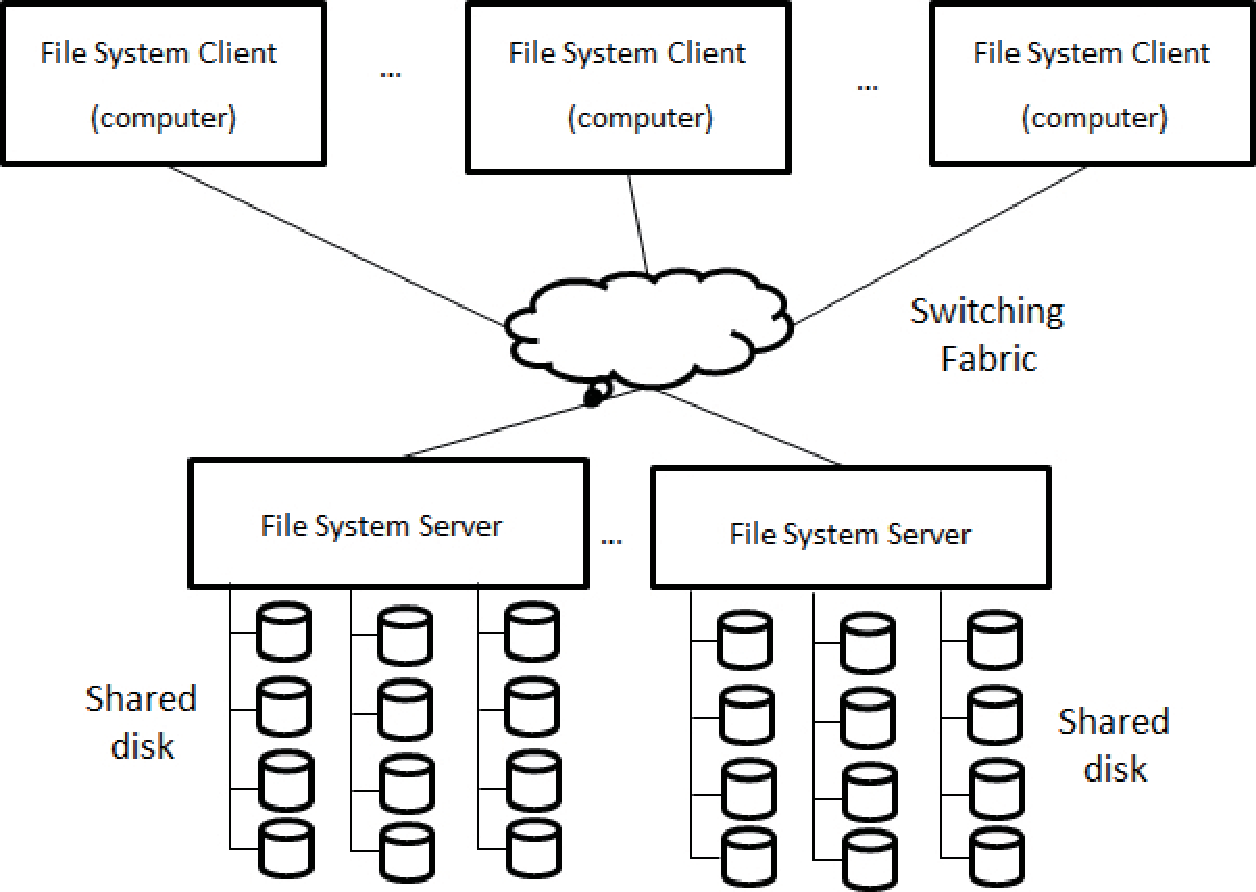
\includegraphics[width=3in]{figures/f13}
\par\end{centering}

\caption{\textbf{GPFS architecture. }}
\label{fig:f13} 
\end{figure}

GPFS provides fault-tolerance in large-scale clusters in three
situations. Upon a node failure, GPFS will restore
metadata updated by the failed node to a consistent state and release
lock tokens in the failed node and appoint others nodes for special
roles played by the failed node. Upon a communication
failure, the mechanism for one node lost is handled as the node failures
while a network equipment failure causes a network partition. In the
case of partition, the nodes in the partition that has the highest
number of nodes have access to the shared disks. GPFS uses data
replication across multiple disks to deal with disk failures. 

Cloud users can deploy a shared-disk file system by installing the corresponding
frameworks (\textit{e.g.} GPFS framework) in the VMs with the cloud
storage resources such as Microsoft Blob Storage and Amazon Elastic
Block Store (EBS). Alternatively, cloud users can mount Amazon Simple
Storage Service (S3) into all the Linux-based VMs to realize the
functionality that all the VMs can have access to the same storage
resource, as with a shared-disk file system.\\
\\
\textbf{Distributed file systems}\\
A distributed file system
stores data directly in the file system that is constructed by gathering
storage space in each computing node in a shared-nothing architecture.
The distributed file system integrates solutions for load
balancing among computing nodes, fault-tolerance and concurrent
access. Files must be partitionned into chunks, \textit{e.g.} through a hash
function on records' keys, and the chunks are distributed among
computing nodes.
Different from the shared-disk file system, computing
nodes have to load the data chunks from the distributed file system to the
local system before local processing. 

Let us illustrate with Google File System (GFS) \cite{Ghemawat2003},
which had a major impact on cloud data management.
For instance, Hadoop Distributed File System (HDFS) is an open source framework
based on GFS.
GFS is designed for a shared-nothing cluster made of commodity
computers, and applications with frequent read operations while
write operations mainly consist of appending new data. 
GFS is composed of a single GFS master node and multiple GFS chunk servers.
The GFS master maintains all the file system metadata while GFS chunk servers
store all the real data. The master can send instruction information to the chunk servers while the chunk server can send chunk server status information to the master. A GFS client can get
the data location information from the file namespace of the GFS master. Then it can write data to the GFS chunk servers at this data location or get the data chunks 
from a corresponding GFS chunk server according to the data location information and required data size. 
This mechanism is shown in Figure \ref{fig:f14}. GFS also provides
snapshot support,
garbage collection, fault-tolerance and diagnosis. For
high availability,  GFS supports master replication and data chunk replication.

\begin{figure}
\begin{centering}
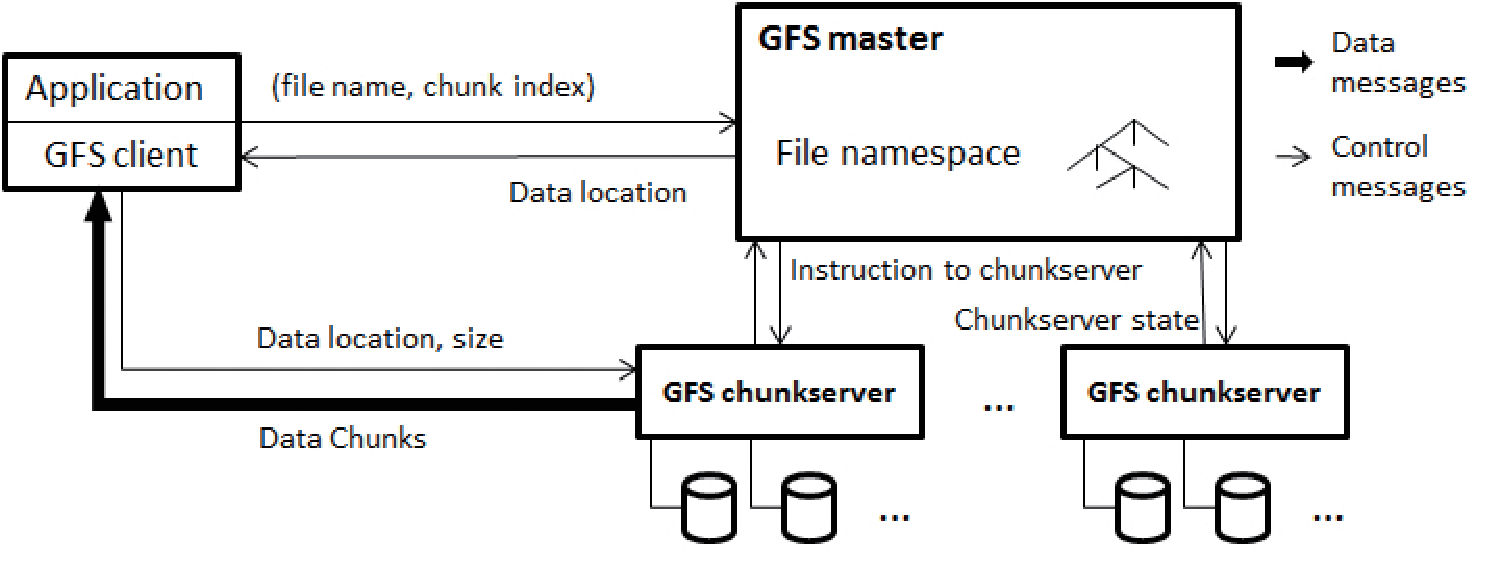
\includegraphics[width=4in]{figures/f14}
\par\end{centering}

\caption{\textbf{GFS architecture \cite{Ghemawat2003}. }}
\label{fig:f14} 
\end{figure}


BlobSeer \cite{Nicolae2011} is another distributed file system
optimized for Binary Large OBjects (BLOBs). 
The architecture of BlobSeer is shown
in Figure \ref{fig:f15}. Data providers
physically store the data in the storage resources (data providers) while physical storage resources can be inserted
or removed dynamically in the data providers. The provider manager tracks the information
about the storage resources and schedules the placement of newly generated
data. All the stored data has a version. Metadata providers store the metadata for identifying data chunks
that make up a snapshot version. The version manager assigns new snapshot version numbers to writers
and appenders and reveals new snapshots to readers. The write operation
is performed in parallel on data chunks and creates a new version of
the data.
Because of data versioning, read and write operations can be
asynchronous and thus
improve the read and write throughput. 
The client can
get the data location of the required files corresponding to the file name and the required version when the required version is
equal or inferior to the latest snapshot version. Then it can write
data to the data providers or get the corresponding data chunks from
the data providers by the data location and desired data
size. BlobSeer also provides
fault-tolerance through replication, consistency semantics
and scalability based on several versioning mechanisms.
Nicolae \textit{et al.} \cite{Nicolae2011} made a first performance comparison of Blobster with HDFS, which shows important improvements in read and write thoughput, because of versioning. 

Cloud users can deploy a distributed file system by installing corresponding frameworks (\textit{e.g.} HDFS) of the aforementioned systems in available VMs to gather storage resources in each VM for executing applications in the Cloud.

\begin{figure}
\begin{centering}
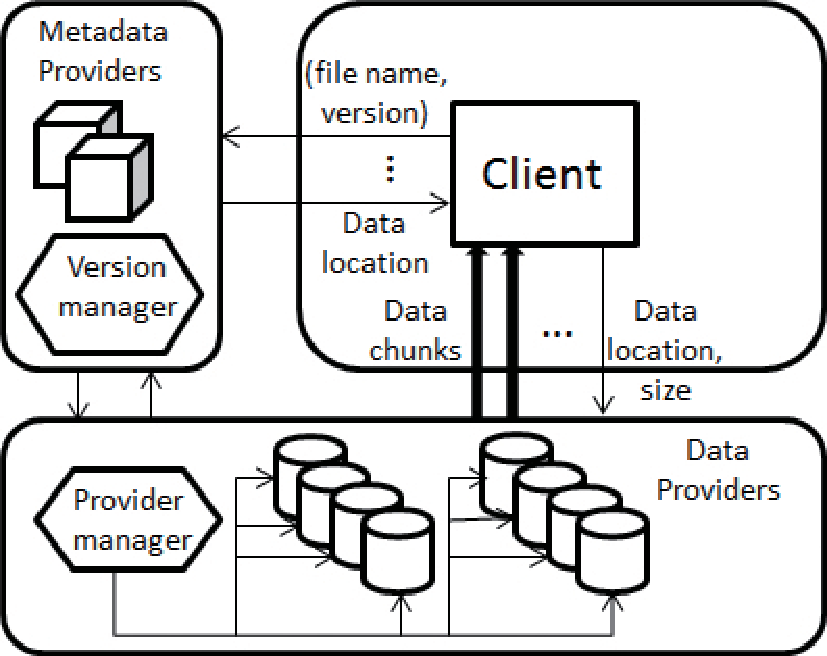
\includegraphics[width=3in]{figures/f15}
\par\end{centering}

\caption{\textbf{BlobSeer Architecture \cite{Nicolae2011}. }}
\label{fig:f15} 
\end{figure}


\subsection{Scientific Workflow Execution in the Cloud}

The cloud has some useful features to execute SWfs. In particular, the quality of service guaranteed by SLA can yield more stable performance. Juve \textit{et al.} \cite{Juve2013} compare the performance
of an astronomy application with the Pegasus SWfMS in the grid, the
commercial cloud and the academic cloud. They conclude that the performance
is the least stable in grid and more stable in commercial cloud
than academic cloud. We present the adaptations of SWfMSs for cloud environments, including SWf execution in a single site cloud and that in multiple cloud sites.


\subsubsection{Execution at a Single Cloud Site}

In a single site cloud environment, SWfMSs can be directly installed in the VMs and exploit services deployed in the cloud \cite{Juve2011,Wolstencroft2013,Deelman2012}. Existing parallelization techniques, \textit{e.g.} parallelism techniques (see Section \ref{sec:subsec:WP}), scheduling techniques (see Section \ref{sec:sub:WS}), existing execution execution models in grid \cite{Deelman2012}, can be used to execute a data-intensive SWf in the environment. 
SWfMSs can exploit some middleware to create or remove VMs and enable the communication between VMs in order to execute data-intensive SWfs in the cloud \cite{Hategan2011,Wang2012,Afgan2010}, such as Coasters \cite{Hategan2011} in Swift, Kepler 
EC$2$ actors \cite{Wang2012} for Kepler, CloudMan \cite{Afgan2010} for Galaxy and 
RabbitMQ$12$ for Triana\footnote{Triana in cloud: \url{http://www.trianacode.org/news.php}} SWfMS. 
These tools can provide computing or storage provisioning for SWf execution or communication 
between VMs. However, they cannot take advantage of the dynamic provisioning features 
of the cloud.

Some SWfMSs can take advantage of the scalability of cloud to provision VMs and storage for SWf execution.
For instance, Afgan \textit{et al.} \cite{Afgan2010} propose CloudMan that
permits Galaxy to make use of Amazon EC2 and EBS for computing and
storage provisioning for SWf execution.
Some other SWfMSs are optimized for the cloud by supporting dynamic resource provisioning under budget and time 
limits, such as Pegasus \cite{Malawski2012,Nagavaram2011} with Wrangler \cite{Juve2011a} 
(a dynamic provisioning system in the cloud) and Askalon \cite{Ostermann2009a,Ostermann2011,Fard2013} SWfMS.
Since high parallelization degree can lead to less execution time, SWfMSs can dynamically create new VMs in order to reduce execution time under monetary cost constraint. But if the estimated monetary cost of SWf execution with current number of VMs exceeds the monetary cost constraint, SWfMSs can remove some VMs. 


Chiron is adapted to the cloud through its extension, Scicumulus \cite{Oliveira2010,Oliveira2012}. 
The architecture of Scicumulus contains three layers and four corresponding tiers: desktop layer 
for client tier, distribution layer for distribution tier, execution layer for 
execution tier and data tier. The desktop layer is to compose and execute SWfs. 
The distribution layer is responsible for parallel execution of activities in the cloud. 
The execution layer manages activity execution in VM instances. Finally, the data tier 
manages the related data during SWf execution. Scicumulus exploits hybrid scheduling approaches 
with dynamic computing provisioning support. Furthermore, Scicumulus uses 
services such as SciDim \cite{Oliveira2013} to determine an initial virtual cluster size 
through a multi-objective cost function and provenance data under budget and time limits. 
Moreover, Scicumulus can be coupled with  SciMultaneous, which is used
to manage fault tolerance in the cloud \cite{Costa2012}. 

\subsubsection{Execution in a Multisite Cloud}

Clouds are independent of geographical distribution of physical resources by nature. However, it is possible to control the location of deployed services for better performance in some cloud environments, \textit{e.g.} Microsoft Azure cloud \cite{MicrosoftAzure} and Amazon cloud \cite{AmazonCloud}.
In general, a user uses a single site, which is sufficient for most applications.
However, there are important cases where SWfs will
need to be deployed at several sites, \textit{e.g.} because the data accessed by
the SWf is in different research groups' databases in different
sites or because SWf execution needs more resources than those at a
single site. Big cloud providers such as Microsoft and Amazon
typically have multiple geographically distributed data centers located at different sites. 
In some cases, a SWf must be executed at multiples sites.
There are two approaches to do this. The first approach is to deploy
a SWfMS in a multisite cloud platform as discussed in
Section \ref{sec:sub:MMC}. The second approach is to make a SWfMS multisite-aware
and capable to utilize computing and storage resources
distributed at different sites. This is the approach we now focus on.

In a multisite cloud, we can execute a SWf with or without SWf partitioning.
SWf execution without partitioning is to schedule all the tasks into all the VMs in the multiple sites. This centralized method makes it hard to realize load balancing, incurs
much overhead for each task and makes scheduling very complicated.
With partitioning, a SWf is divided in fragments
(see Section \ref{sec:subsec:WP}) and each fragment is scheduled at a specific
site and its tasks scheduled within the VMs at this site. 
This method can reduce the overhead of task scheduling, which is done
in parallel at multiple sites, and realize load balancing at two
levels: inter-site and intra-site.
Inter-site load balancing is realized by scheduling fragments,
with a global scheduler,
and intra-site load balancing is realized by local task scheduling. 
This two-level approach makes the scheduling operation
easier. 

Swift and Pegasus achieve multisite execution by SWf partitioning. Swift performs SWf partitioning by generating
corresponding abstract WEPs for each site \cite{Zhao2007}.
Pegasus realizes partitioning through several methods
\cite{Chen2012a, Chen2013}. As discussed in Section \ref{sec:subsubsec:WGL}, Chen and Deelman
\cite{Chen2012a} propose a SWf partitioning method under storage
constraints at each site. This SWf partitioning method is used in a multisite environment with dynamic computing provisioning as explained in \cite{Chen2012}.
Another method is balanced task clustering \cite{Chen2013}.
The SWf is partitioned into several fragments which have almost the same workload.
This method can realize load balancing for homogeneous computing
resources. Askalon can execute SWf in
a federated multisite cloud \cite{Ostermann2009a}, \textit{i.e.} a multisite cloud composed of resources from different providers.
Nevertheless, it schedules tasks in computing nodes 
without considering the organization of computing resources,
\textit{i.e.} which VMs are at the same site, for optimization. 
This method just takes the VMs as the grid computing nodes without considering the features of multisite resources, \textit{e.g.}
the difference of data transfer rate, resource sharing for intra-site and inter-site, etc.

\subsection{Conclusion and Remarks}

There are important cases where SWfs will need to be
deployed at several data centers in the cloud, either from the same or
different cloud providers, thus making multisite management an important problem.
Although some SWfMSs such as Swift and Pegasus provide some
functionality to execute SWfs in the multisite environment, this is generally done
by simply reusing the techniques from a grid environment or simple dynamic provisioning and scheduling mechanisms, without
exploiting new data storage and data transfer capabilities provided by
multisite clouds. 

We believe that much more work is needed to improve the execution of
data-intensive SWfs in a multisite cloud.
First, the co-scheduling of tasks and data should be exploited.
Most SWfMSs make use of a shared file system to store data
but do not care about where the data is stored for task scheduling.
We believe that the co-scheduling of tasks and data can be efficient
at maximizing local data processing.
Second, SWfMSs could optimize the task scheduling while ensuring provenance support with the consideration of different bandwidths among different sites. 
Third, the communication between two sites is generally achieved by
having two nodes, each at one of the two sites, communicating
directly, which is not efficient in a multisite cloud. For instance, 
selecting several nodes at one site to send
or receive data to or from several nodes at another site could exploit
parallel data transfer and make it more efficient.




\section{Overview of Existing Solutions}
\label{sec:SOAOES}

In this section, we illustrate SWf parallel execution solutions in existing SWfMSs. 
This section starts by a short presentation of parallel
processing frameworks such as MapReduce. Although they are not
full-fledged SWfMS, they do share techniques in common and
are often used for complex scientific data analyses, or in conjunction
with SWfMS to deal with big data \cite{Wang2009}. Then, the section introduces eight widely used SWfMSs and a science gateway platform. Finally, the section ends with concluding remarks.

\subsection{Parallel Processing Frameworks}

Parallel processing frameworks enable the programming and execution of
big data analysis applications in massively parallel computing infrastructures.

MapReduce \cite{Dean2004} is a popular parallel processing framework
for shared-nothing clusters, \textit{i.e.} highly-scalable clusters with no sharing of either
disk or memory among computers.
MapReduce was initially developed by Google as a proprietary product
to process large amounts of unstructured or semi-structured data, such
as web documents and logs of web page requests, on large
shared-nothing clusters of commodity nodes and produce various kinds
of data such as inverted indices or URL access frequencies. Different
implementations of MapReduce are now available such as Amazon
MapReduce (as a cloud service) or Hadoop \cite{White2009}.

MapReduce includes only two types of operations, \emph{map} and
\emph{reduce}. The Map operation is applied to each
record in the input data set to compute one or more intermediate
(key,value) pairs. The Reduce operation is applied to all the values
that share the same unique key in order to compute a combined
result. Since they work on independent inputs, Map and Reduce can be
automatically processed in parallel, on different data chunks
using many computer nodes in a cluster. 

MapReduce execution proceeds as follows (see Figure \ref{fig:f7}).
First, the users submit their jobs composed of  MapReduce functions to a scheduling system. 
When the user program calls the MapReduce job, the MapReduce library in the user program splits the input data into several chunks.
A MapReduce job consists of one Map function and one Reduce function.
Then, the library makes several copies of the functions and distribute the copies into available computers. 
One copy is the master while the others are workers that
are assigned tasks by the master. 
The master attempts to schedule a Map task, which is composed of a copy of the map function and corresponding input data chunks, to an idle worker. 
The worker that is assigned a Map task processes the (key,value)
pairs of input data chunks and puts the intermediate (key,value)
pairs in memory. 
The intermediate data is written to local disk periodically
after being partitioned into several regions and the location information of this data is passed to the master. 
The combination of a copy of Reduce function and related intermediate data chunks is a Reduce task.
The worker, which is assigned a Reduce
task, reads the corresponding intermediate (key,value) data and sorts the data by grouping the data of the
same key together. Then the sorted data is passed to 
Reduce tasks, which process the data and append their output data to a final output file. 
When all the map tasks and reduce tasks are completed, the master wakes up the user program.


\begin{figure}
\begin{centering}
\captionsetup{justification=centering}
\includegraphics[width=129mm]{figures/f7}
\par\end{centering}

\caption{\textbf{MapReduce execution process. }}
\label{fig:f7} 
\end{figure}


Hadoop is an open source framework that supports MapReduce in a shared-nothing cluster.
It uses Hadoop Distributed File System (HDFS) as storage layer
(see Section \ref{sec:sub:MMC}). In Hadoop, MapReduce programs take
input data from HDFS and put the final result and execution logs back
to HDFS. Using Hadoop framework for SWf parallel execution can
facilitate the implementation of SWfMSs and offer good compatibility
for MapReduce programs.
Hadoop is extended to multiple sites while the existing approaches do not consider the provenance support or different bandwidths among different sites for the task scheduling \cite{Wang2013}. However, Hadoop can be used for executing SWfs by with combination of SWfMSs.
For instance, Wang \textit{et al.}
\cite{Wang2009} propose an architecture that combines
Kepler with Hadoop so that Kepler can represent an activity as a
MapReduce program and exploit the Hadoop framework to execute tasks. While
designing a SWf with MapReduce activities, the input
path, output path and result for the MapReduce activities should be
specified through the Kepler GUI. Inside of the MapReduce activity, the
input key, input value (input list) and output list (or output value) for the
Map function (or Reduce function) should be specifed through the
GUI. During the execution of a MapReduce activity in the Kepler/Hadoop
system,
Kepler first transfers all the input data into
HDFS. Then, it runs the Map function followed by the Reduce function in the
Hadoop system.
Finally, it retrieves the output
data from HDFS and stores it to the local file system.
This approach enables Kepler to
outsource data parallelism of a MapReduce activity to Hadoop, yet
loosing control of activity execution.


\textit{Pig} \cite{Olston2008} is 
an interactive, or script-based, execution environment atop MapReduce. 
It supports \textit{Pig Latin},  a declarative worflow language to
express large dataset analysis.
PigLatin resembles SQL, with a more procedural style, and allows
expressing sequences of activities that get translated in MapReduce jobs.
Pig Latin can be extended using user-defined functions
written in different languages like Java, Python or JavaScript.
Pig programs can be run in three different ways: with a script
interpreter, with a command interpreter or embedded in a Java program.
Pig performs some logical optimization, by grouping activities into
MapReduce jobs. For executing the activities, Pig
relies on Hadoop to schedule the corresponding Map and Reduce tasks.
Hadoop provides the functionality such as 
load-balancing and fault-tolerance. However, task scheduling and data dispatching in 
Hadoop is not optimized for the entire SWf. 

Dryad \cite{Isard2007} is another parallel processing framework
developed by Microsoft (which eventually adopted Hadoop MapReduce).
Similar to a SWf, a Dryad job is represented as a DAG. 
To compose a Dryad job, the users can extend Dryad by implementing new composition operations based
on two standard compositions: $A>=B$ and $A>>B$ (see Figure \ref{fig:f8}). 
During job execution, Dryad refines the job graph in order to reduce
network consumption. Once all the input data of one program (vertex) is
ready, the corresponding programs (vertices) are put into a scheduling
queue, which applies a greedy scheduling strategy.
Then, Dryad re-executes corresponding failed programs several times for fault tolerance.

\begin{figure}
\begin{centering}
\captionsetup{justification=centering}
\includegraphics[width=129mm]{figures/f8}
\par\end{centering}

\caption{\textbf{Dryad operations \cite{Isard2007}. } Circles represent programs
and arrows represent data dependencies. Box (a) and box (b) illustrate
program cloning with the \textasciicircum{} operator. We note each program
$P$ of type $x$ as $P_x$. The
operation $AS>=BS$ in (c) means that each $P_a$
has an input data flow to each $P_b$. The operation
$AS>>BS$ in (d) expresses complete
bipartite composition. Box (e) shows an operation by combining
the data from $Pb$ to $P_c$
and $P_d$.}
\label{fig:f8} 
\end{figure}

\subsection{SWfMS}
Most SWfMSs implement the five layer architecture discussed in Section \ref{sec:sub:FAS}.
We selected eight typical SWfMSs and a gateway framework to illustrate their techniques: Pegasus,
Swift, Kepler, Taverna, Chiron, Galaxy, Triana \cite{Taylor2007}, Askalon \cite{Fahringer2007} and WS-PGRADE/gUSE \cite{Kacsuk2012}. 
Pegasus and Swift have excellent support for scalability and high-performance of data-intensive SWfs, with reported results using more than a hundred thousand of cores and terabytes of data during SWf execution \cite{Deelman2014,Zhao2007}.
Kepler, Taverna, Triana have a GUI for
desktop computers. Chiron is widely used because of a powerful algebraic approach for SWf parallelization. 
Galaxy integrates a GUI that can
be accessed through web browsers. Triana is able to use P$2$P services. 
Askalon implements both desktop and web GUI and has been adapted to cloud environments.
WS-PGRADE/gUSE is a widely used gateway framework, which enables SWf execution in Distributed Computing Infrastructures (DCI) with a web interface for users. 


Pegasus, Swift, Kepler, Taverna and WS-PGRADE/gUSE are widely used in astronomy, biology, and so on while Galaxy can only execute bioinformatics SWfs.
Pegasus, Swift and Chiron design and execute a SWf
through a textual interface while Kepler, Taverna, Galaxy, Triana, Askalon and WS-PGRADE/gUSE integrate a GUI for SWf design.
All of the eight SWfMSs and the gateway framework support SWf specification in a DAG
structure while Swift, Kepler, Chiron, Galaxy, Triana and Askalon also support SWfs in a DCG structure \cite{Yu2005}.
Users can share SWf information from Taverna, Galaxy, Askalon and WS-PGRADE/gUSE. 
All of them support independent parallelism. 
All of them support dynamic scheduling and three of them (Pegasus, Kepler and WS-PGRADE/gUSE) support static scheduling. All the eight SWfMSs and the gateway framework support SWf execution in both grid and cloud environments.
A brief comparison of these eight SWfMSs and the gateway framework is given in Table \ref{tab:sim}. 

\subsubsection{Pegasus} 

Pegasus%
\footnote{Pegasus: http://pegasus.isi.edu/%
} \cite{Deelman2014} is widely used in multiple disciplines such as astronomy,
bioinformatics, climate modeling, earthquake science, genome analysis, etc. 
Pegasus has interesting features: portability on different infrastructures such as grid and cloud,
optimized scheduling algorithms; good scalability,
support for provenance data that can be used for debugging,
data transfer support for data-intensive SWfs,
fault-tolerance support, detailed user guide \cite{PegasusUserGuide} and available package in the Debian repository.


Pegasus consists of five components, \textit{i.e.} mapper, local execution engine, job scheduler, remote execution engine and monitoring component. 
The mapper generates an executable SWf and partitions SWf to fragments based on an abstract SWf provided by the users.
The local execution engine submits the fragments to execution engines according to dependencies.
The job scheduler schedules the fragments to available remote execution engines.
The remote execution engine manages the execution of the tasks of the fragments. 
Finally, the monitoring component monitors the execution of the SWf.

The process of executing SWfs in Pegasus is shown in
Figure \ref{fig:f10}. In the presentation layer, Pegasus takes an 
abstract SWf represented as a DAX (DAG in an XML file).
Pegasus provides programmatic APIs in Python, Java, and Perl for DAX generation\cite{PegasusUserGuide}. Pegasus exploits a lightweight web dashboard to monitor and the execution of SWfs for a user.
In the user services layer, Pegasus supports SWf monitoring through Stampede monitoring infrastructure \cite{Gunter2011,Samak2011}. 
Pegasus also support provenance data gathering and
\begin{landscape}
\begin{table}
\caption{\textbf{Comparison of SWfMSs. }A categorization of SWfMSs based
on supported SWf structures, SWf information sharing, UI types, 
parallelism types and scheduling methods. \textquotedblleft{}activity\textquotedblright{} 
means that this SWfMS supports both independent parallelism and pipeline parallelism. WPg represents WS-PGRADE/gUSE. WP indicates that the interface is a web-portal.}
\label{tab:sim}
\begin{centering}
\captionsetup{justification=centering}
\begin{tabular}{cccccc}
\hline 
SWfMS & structures & SWf sharing & UI type & parallelism & scheduling \tabularnewline
\hline 
Pegasus & DAG & not supported & GUI \& textual & data \& independent & static \& dynamic \tabularnewline
Swift & DCG & not supported & textual & activity & dynamic \tabularnewline
Kepler & DCG & not supported & GUI & activity & static \& dynamic \tabularnewline
Taverna & DAG & supported & GUI & data \& activity & dynamic \tabularnewline
Chiron & DCG & not supported & textual & data \& activity \& hybrid & dynamic \tabularnewline
Galaxy & DCG & supported & GUI (WP) & independent & dynamic \tabularnewline
Triana & DCG & not supported & GUI & data \& activity & dynamic \tabularnewline
Askalon & DCG & supported & GUI  & activity & dynamic \& hybrid \tabularnewline
WPg & DAG & supported & GUI (WP) & data \& independent \& hybrid & static \& dynamic \tabularnewline
\hline 
\end{tabular}
\par\end{centering} 
\end{table}
\end{landscape}
\begin{figure}
\begin{centering}
\captionsetup{justification=centering}
\includegraphics[width=129mm]{figures/f10}
\par\end{centering}
\caption{\textbf{Pegasus SWf execution process \cite{Deelman2005}. }}
\label{fig:f10} 
\end{figure}
\noindent querying through a Pegasus/Wings framework \cite{Kim2008}. The provenance data or monitoring data come from the log data gathered during SWf execution.

In the WEP generation layer, the mapper reduces the abstract SWf by checking available intermediate data in the available computing nodes. The intermediate data can come from the previous execution of the same 
SWf or the execution of other SWfs that contain several common activities. 
In addition, Pegasus inserts the data transfer activities, \textit{e.g.} data stage-in, in the DAG for SWf execution. 
The mapper component can realize SWf partitioning through three methods
\cite{Chen2012a,Chen2013,Deelman2014}. As discussed in Section \ref{sec:subsubsec:WGL}, Chen and Deelman \cite{Chen2012a} propose a SWf partitioning method under storage constraints at each site. This partitioning method is used in a multisite environment with dynamic computing provisioning as explained in \cite{Chen2012}.
Another method is balanced task clustering \cite{Chen2013}.
The SWf is partitioned into several fragments which have almost the same workload. This method can realize load balancing for homogeneous computing resources. 
The last method is to cluster the tasks of the same label \cite{Deelman2014}.
To use this method, the tasks should be labeled by users.
In the WEP execution layer, the job scheduler may perform site execution based on standard algorithms (random, round-robin and min-min),
data location and the significance of computation and data in SWf execution. For example, the job scheduler moves computation to the data site where big volume of data is located and it sends data to compute site if computation is significant. 
At this point, Pegasus schedules the execution of tasks within a SWf engine such as DAGMan.  
In Pegasus, DAGMan sends the concrete executable tasks to Condor-G, a client tool
that can manage the execution of a bag of related tasks on grid-accessible computation nodes in the selected sites. 
Condor-G has a queue of tasks and it schedules a task in this queue to a computing node in the selected site once this computing node is idle \cite{Frey2001,Litzkow1988}. 
Pegasus handles task failures by retrying the corresponding part of SWfs or transfer the data again with a safer data transfer method. 
Through these mechanisms, Pegasus hides the complex scheduling, optimization and data transmission of SWfs from SWfMS users.

In the infrastructure layer, Pegasus is able to use computing cluster, grid (including desktop grids) and cloud to execute a SWf. 
It can exploit a shared file system, local storage resources at each computing node or cloud storage, \textit{e.g.} Amazon S$3$, for data storage and it provides static computing and storage provisioning for SWf execution. Pegasus can be directly executed in a virtual cluster in cloud \cite{Juve2011} while it can also use dynamic scheduling algorithms \cite{Malawski2012,Nagavaram2011} for budget constraint and time limit through Wrangler \cite{Juve2011a}, a dynamic provisioning system in the cloud.

\subsubsection{Swift}
Similar to Pegasus, Swift \cite{Zhao2007} has been used in multiple disciplines such as biology,
astronomy, economics, neuroscience, etc. Swift grew out of the GriPhyN
Virtual Data System (VDS) whose objective is to express, execute,
track the results of SWfs through program optimization and
scheduling, task management, and data management. Swift has been revised and 
improved its (already) large-scale performance into the Turbine system \cite{Wozniak2012}.

Swift executes data-intensive SWfs
through five functional phases: program specification, scheduling,
execution, provenance management and provisioning.
In the presentation layer, Swift takes a SWf specification that
can be described in two languages: XDTM and SwfitScript.
XDTM is an interface to map the logical structure of data to physical
resources. SwiftScript defines the sequential or parallel computational procedures that operate
on the data defined by XDTM. 
In the user services layer, provenance data is available for the users.

In the WEP generation layer, the SwiftScript is compiled
to an abstract computation specification. Swift performs partitioning by generating corresponding abstract WEPs for each site \cite{Zhao2007}.
In the WEP execution layer, the abstract WEPs are scheduled to execution sites.
The Karajan SWf execution engine is used by Swift to realize the functions such as data transfer, task
submission, grid services access, task instantiation, and task schedule. 
Swift runtime callouts provide the information for task and data scheduling and
offer status reporting, which shows the SPs. 
During SWf execution,
provenance data is gathered by a launcher program (\textit{e.g.} kickstart). Swift achieves fault tolerance by retrying the failed tasks
and provides a restart log when the failures are permanent.

In the infrastructure layer, the provisioning phase of Swift provides computing resources in a computer cluster, grid, and cloud through a dynamic resource provisioner for each execution site. 
In the cloud, Swift takes advantage of Coasters \cite{Hategan2011} to manage communication, task allocation and data stage for scientific SWf execution while it is not optimized for dynamic provisioning of VMs and storage. 
Figure \ref{fig:f11} depicts the Swift system architecture.

\begin{figure}
\begin{centering}
\captionsetup{justification=centering}
\includegraphics[width=129mm]{figures/f11}
\par\end{centering}

\caption{\textbf{Swift system architecture \cite{Zhao2007}. }}
\label{fig:f11} 
\end{figure}


\subsubsection{Kepler}
Kepler \cite{Altintas2004,Altintas2004a} is a SWfMS built upon the Ptolemy
II system from the Kepler%
\footnote{Kepler project: https://kepler-project.org/%
} project. It allows to plug in different execution models into SWfs.
Kepler is used in many projects of various disciplines such as oceanography%
\footnote{REAP project: https://kepler-project.org/users/projects-using-kepler-1/reap-project%
}, data management%
\footnote{Scientific Data Management Center: https://sdm.lbl.gov/sdmcenter/%
}, and biology%
\footnote{Clotho project: http://www.clothocad.org/%
} etc. Kepler integrates a powerful graphical workbench (shown in Figure \ref{fig:f12}).
In the presentation layer, each individual reusable SWf step
is implemented as an actor that can be signal processing, statistical
operations, etc. SWf activities are associated to different actors as shown in Figure \ref{fig:f12}. 

In the user services layer, the provenance functionality in Kepler is realized
by corresponding actors such as Provenance Recorder (PR)
\cite{Altintas2006}. PR records the information of SWf execution
such as context, input data, associated metadata, SWf
outputs, etc. 

In the WEP generation layer, the SWf is handled by a separate component named director.
Kepler supports several directors and each director corresponds to a unique model of execution, which is a model of WEP. 
The director generates executable tasks to achieve activity parallelism (pipeline parallelism and independent parallelism).

In the WEP execution layer, Kepler exploits static or dynamic scheduling according to the director that is used during SWf execution \cite{Ludascher2006,Bux2013}.
The fault tolerance functionality of Kepler can be achieved
by a framework that provides three complementary mechanisms. The first
mechanism is a forward recovery mechanism that retries the failed
tasks. The second mechanism offers a check-pointing mechanism that
resumes the execution in case of a failure at the last saved 
state. The last one is a watchdog process that analyzes the SWf
execution based on provenance data and sends an appropriate signal
and possible course of action to the SWf engine to handle it. 
Kepler executes SWfs in parallel through web services, 
grid-based actors or Hadoop framework.
Kepler can execute SWfs by using external execution environments such as SAS, Matlab,
Python, Perl, C++ and R (S+) using corresponding actors.

In the infrastructure layer, Kepler can achieve data access through an OpenDBConnection actor for data in a database and an EMLDataSource actor for ecological and biological datasets. Kepler is compatible with the cloud through Kepler EC$2$ actors, which can directly create a set of EC$2$ VMs and attach Elastic Block Store volumes to running VMs \cite{Wang2012}. 

\begin{figure}
\begin{centering}
\captionsetup{justification=centering}
\includegraphics[width=129mm]{figures/f12}
\par\end{centering}

\caption{\textbf{Kepler workbench. }}
\label{fig:f12} 
\end{figure}

\subsubsection{Taverna}
Taverna \cite{Missier2010} is an open-source SWfMS from the
$^{my}$Grid project to 
support workflow-based biological experiments.
Taverna is used in multiple areas such as astronomy, bioinformatics, chemistry etc. 
In the presentation layer, Taverna takes a GUI
for designing SWfs and 
showing monitoring information while it uses a textual language to represent a 
SWf as a DAG \cite{Yu2005}. 
The SWfs can be designed in Taverna installed in the user's computer or an online web server.
Moreover, this GUI can be installed in an Android mobile \cite{Zhang2013} 

In the user services layer, Taverna uses a state machine for the activities to achieve SWf monitoring \cite{Oinn2004}.
The SWfs designed through Taverna can be shared through \textquotedblleft{}myExperiment\textquotedblright{} social network \cite{Wolstencroft2013}.
It gathers provenance data from local execution information and the remotely invoked web services \cite{Oinn2007}. 

In the WEP generation layer, Taverna automatically optimizes the SWf structure by identifying complex 
parts of structures and simplifies them for easier design and parallelization \cite{Cohen-Boulakia2014}. 
Taverna links the invocation of web services and the 
activities and checks the availability of the needed web services for generating a WEP.
In the WEP execution layer, Taverna relies on web and grid services for task execution. 

In the infrastructure layer, Taverna is able to use the computing resources from grid or cloud. It also stores execution data in a database.

\subsubsection{Chiron}
Chiron exploits a database approach \cite{Ozsu2011} to manage the parallel execution of data-intensive SWfs. 
In the presentation layer, it uses an algebraic data model to express all data as relations and represent SWf activities as algebraic expressions in the presentation layer. 
A relation contains sets of tuples composed of basic attributes such
as integer, float, string, and file references, etc.
An algebraic expression consists of algebraic
activities, additional operands, operators, input relations and output relations.
An algebraic activity contains a program or an SQL expression, and input
and output relation schemas. 
An additional operand is the side information for the algebraic expression, which can be relations
or a set of grouping attributes.
There are six operators:
Map, SplitMap, Reduce, Filter, SRQuery and MRQuery (see Section
\ref{sec:subsub:PL} for the function of each operator). 
In the user services layer, Chiron supports SWf monitoring, steering and gathers provenance data based on algebraic approach. 

In the WEP generation layer, a SWf is wholly expressed in an XML file called conceptual model. 
Chiron supports all types of parallelism (data parallelism, independent parallelism,
pipeline parallelism, hybrid parallelism) and optimizes SWf scheduling
by distinguishing between blocking activities, \textit{i.e.} activities that require all their input data to
proceed, and non blocking, \textit{i.e.} that can be pipelined.
Chiron generates concrete executable tasks for each activity and schedules the tasks
of the same fragments to multiple computing nodes.
Chiron uses two scheduling policies, called blocking and pipeline in \cite{Dias2013}. 
Let \textit{A} be a task that produces data consumed by a task \textit{B}.
With the blocking policy, \textit{B} can start only after all the data produced by \textit{A} are ready.
Hence, there is no parallelism between \textit{A} and \textit{B}.
With the pipeline policy, \textit{B} can start as soon as some of its input data chunks are ready. 
Hence, there is pipeline parallelism.
This pipeline parallelism is inspired by DBMS pipeline parallelism in \cite{Ozsu2011}.
Moreover, Chiron takes advantage of algebraic approach for SWf execution optimization to generate a WEP.

In the WEP execution layer, Chiron uses an execution module file
to specify the scheduling method, database information and input data information. 
Chiron exploits dynamic scheduling method for task execution.
Chiron gathers execution data, light domain data and provenance data into a database structured by following the PROV-Wf \cite{Costa2013} provenance model.
The execution of tasks in Chiron is based on MPJ \cite{Carpenter2000}, an MPI-like message passing
system.
In the infrastructure layer, Chiron exploits a shared-disk file system and database for data storage.  

Chiron is adapted to the cloud through its extension, Scicumulus \cite{Oliveira2010,Oliveira2012}, which supports dynamic computing provisioning \cite{Oliveira2012a}. The architecture of Scicumulus contains three layers and four corresponding tiers: desktop layer 
for client tier, distribution layer for distribution tier, execution layer for execution tier and data tier. The desktop layer is to compose and execute SWfs. The distribution layer is responsible for parallel execution of activities in the cloud. 
The execution layer manages activity execution in VM instances. Finally, the data tier manages the related data during SWf execution. Scicumulus exploits hybrid scheduling approaches 
with dynamic computing provisioning support. Furthermore, Scicumulus uses services such as SciDim \cite{Oliveira2013} to determine an initial virtual cluster size through a multi-objective cost function and provenance data under budget and time limits. Moreover, Scicumulus can be coupled with  SciMultaneous, which is used to manage fault tolerance in the cloud \cite{Costa2012}. 


\subsubsection{Galaxy}
Galaxy is a web-based SWfMS for genomic research. 
In the presentation layer, Galaxy provides a GUI for designing SWfs through browsers. 
It can be installed in a public web server (https://usegalaxy.org/) or a private server to address specific needs. 

In the user services layer, users can upload data from a user's computer or online resources and share SWf information including SWfs, SWf description information, SWf input data and SWf provenance data in a public web site. 
Moreover, users can import SWfs from the \textquotedblleft{}myExperiment\textquotedblright{}
\cite{Wolstencroft2013} social network \cite{Goecks2012}. 

In the WEP generation layer, Galaxy manages the dependencies between each activity for parallelization. 
In the WEP execution layer, Galaxy generates concrete tasks for each activity, 
puts the tasks in a queue to be submitted, and monitors the task status (in queue, running or completion) \cite{Karuna2012}. 
Through this mechanism, Galaxy exploits dynamic scheduling to dispatch executable tasks.
Galaxy uses Gridway to execute tasks in the Grid. 
Gridway manages a task queue and the tasks in a queue are executed in
an available computing node that is selected according to a greedy
approach, \textit{i.e.} requests are sent to all the available computing nodes while the node that has minimum response time is selected \cite{Huedo2004}. 

In the infrastructure layer, Galaxy can exploit Globus \cite{Liu2012} and CloudMan \cite{Afgan2010} to achieve dynamic computing and storage provisioning such as dynamic VM inserting and removing and shared-disk file system construction across computing nodes. Galaxy is adapted to cloud environment by CloudMan \cite{Afgan2010} middlewear, which can create Amazon EC$2$ clusters based on a Bio-Linux machine image, dynamically change cluster size and attach S$3$ storage to the clusters. 

\subsubsection{Triana}
Triana \cite{Taylor2007} is a SWfMS initially developed as a data
analysis tool within the GEO $600$ 
project\footnote{http://www.geo600.org/}. It provides a GUI in the presentation 
layer. In the user services layer, it implements the Stampede monitoring 
infrastructure \cite{Vahi2012} (see Section \ref{sec:subsub:USL}).
 
In the WEP generation layer, Triana exploits components to realize different data 
processing functions similar to Kepler actors.  
In the WEP execution layer, Triana supports the grid Application Toolkit (GAT) API for developing grid-oriented 
components. Triana also uses the Grid Application Prototype (GAP) as an interface to interact 
with service-oriented networks. The GAP contains three bindings, \textit{i.e.} implemented GAP, such as P$2$PS and JXTA 
to use P$2$P network and Web services binding to invoke Web
services. 

In the infrastructure layer, Triana can employ computing resources in the grid or cloud.
Triana uses RabbitMQ12 \footnote{Triana in cloud: \url{http://www.trianacode.org/news.php}}, a message broker platform, to realize the communication among different VMs in order to run SWfs in the cloud environment.

\subsubsection{Askalon}
Askalon \cite{Fahringer2007} is also a SWfMS initially designed for a grid environment. 
In the presentation layer, it provides a GUI, through which a SWf can be modeled using Unified Modeling Language. It also exploits an XML-based language to model workflows.
In the user services layer, it provides on-line SWf execution monitoring functionality
through SWf execution monitoring and dynamic workflow steering to
deal with exceptions in dynamic and unpredictable execution environments
\cite{Prodan2007}.

In the WEP generation layer, Askalon optimizes the SWf representation with loops, \textit{i.e.} within DCG structures, to 
a DAG SWf structure. 
In the WEP execution layer, Askalon exploits an execution engine to provide fault-tolerance at the levels of workflow, activity and control-flow. 
It can exploit static and hybrid scheduling, \textit{e.g.} rescheduling because of unpredictable changes in the execution environment.

In the infrastructure layer, Askalon uses a resource manager to discover and reserve available resources and to deploy executable tasks in the grid environment. Askalon is able to execute SWfs in cloud environment by dynamic creation of VMs with available cloud images \cite{Ostermann2009a}.  In the cloud environment, Askalon can estimate the cost of SWf execution by simulation \cite{Ostermann2011} and provide dynamic resource provisioning and task scheduling under budget constraint \cite{Fard2013}. 

Moreover, Askalon can execute SWfs in a federated multisite cloud \cite{Ostermann2009a}, \textit{i.e.} a multisite cloud composed of resources from different providers.
Nevertheless, it schedules tasks in computing nodes 
without considering the organization of computing resources,
\textit{i.e.} which VMs are at the same site, for optimization. 
This method just takes the VMs as the grid computing nodes without considering the features of multisite resources, \textit{e.g.}
the difference of data transfer rate, resource sharing for intra-site and inter-site, etc.

\subsubsection{WS-PGRADE/gUSE}

WS-PGRADE/gUSE is a science gateway framework widely used in various
disciplines such as biology \cite{Gesing2014}, seismology
\cite{Kocair2014}, astronomy \cite{Sciacca2014}, and neuroscience
\cite{Shahand2014}. It is an open source software
\cite{Kacsuk2012} used for teaching \cite{Olabarriaga2014}, research
\cite{Kiss2014} and commercial activities \cite{Kiss2014a}.


The architecture of WS-PGRADE/gUSE framework is shown in Figure
\ref{fig:f18}. WS-PGRADE portal is a web-portal interface to help
the users designing SWfs. The grid and cloud
User Support Environment (gUSE) is a middle layer for different user
services. The DCI bridge is a web service based application that provides
access to divers infrastructures such as grid and cloud
\cite{Kacsuk2012}.

In the presentation layer, the WS-PGRADE
portal \cite{Kacsuk2011} has a web browser based interface, which
supports the definition of different kinds of SWfs,
including meta-workflows and parameter sweep workflows. The
meta-workflows can contain embedded SWfs, which are supported by the
SHIWA repository, as sub-workflows. In the user services layer,
WS-PGRADE supports SWf information sharing between the users of
%break%
WS-PGRA-DE/gUSE through a build-in SWf repository, which enables
publishing, searching and downloading programs, SWf designs and
templates \cite{Balasko2014}. A SWf template is an available
SWf pattern that can be changed to other SWfs by modifying
corresponding parameters. In addition, it can exploit the SHIWA repository
\cite{Plankensteiner2013} to support SWf sharing between the
users of different SWfMSs. The monitoring functionality is supported
by the gUSE services. However, the framework lacks provenance
support.


In the WEP generation layer, a SWf is represented in
XML format. The framework may use data and independent
parallelism according to the structure of the
SWf \cite{Balasko2014}. The DCI
bridge dynamically schedules the tasks through a submit queue. The
task execution is handled by web services enabled by a web container,
\textit{e.g.} Tomcat or Glassfish.


Provisioning and data storage are provided by the
DCI Bridge \cite{Kacsuk2014}
and CloudBroker framework.
The DCI Bridge can dynamically create VMs through existing images
and cloud configurations.  The CloudBroker is able to
exploit resources distributed in multiple clouds
\cite{Farkas2014}, including major cloud types , \textit{e.g.} Amazon,
OpenStack \cite{Jackson2012} and OpenNebula
\cite{Milojicic2011}. Moreover, it can take advantage of GPUs to
execute the SWfs that invoke GPU programs \cite{Balasko2014}.


\begin{figure}
\begin{centering}
\captionsetup{justification=centering}
\includegraphics[width=84mm]{figures/f18}
\par\end{centering}

\caption{\textbf{Architecture of WS-PGRADE/gUSE \cite{Gottdank2014}. }}
\label{fig:f18} 
\end{figure} 

The SHIWA simulation platform enables reusing of SWfs in ten
different SWfMS environments \cite{Tersty2014}. First, the users can
search for SWfs in the SHIWA
repository, where SWf developers can upload available programs or
SWfs. Then, the SWfs can be downloaded and adjusted to an Interoperable Workflow Intermediate
Representation (IWIR) language to compose a meta-workflow
\cite{Plankensteiner2013}. Then, when the meta-workflow is
submitted in the platform, each sub-workflow of the
meta-workflow can be scheduled to the appropriate  SWfMS execution environment.


\subsection{Concluding Remarks}

We observed that some SWfMSs take advantage of parallel processing
frameworks such as Hadoop as lower-level tools
to parallelize SWf execution and schedule tasks. This is a
straightforward approach to extend a SWfMS with parallel processing capabilities. However, it lacks the capability to perform parallelization according to the entire SWf structure.
Our comparative presentation of eight SWfMSs showed that most SWfMSs do
not exploit hybrid parallelism (only Chiron does) and hybrid scheduling methods (only Askalon does), which may bring the highest degrees of parallelism and good load balancing.

Although there has been much work on data-intensive SWf management, we believe there is a lot of room for improvement.
First, input data staging needs more attention. Most SWfMSs just do
this as a preprocessing step before actual SWf execution.
For data-intensive SWfs, this step may take a very
long time, for instance,
to transfer several gigabytes to a computing node.
Integrating this step as part of the WEP can help optimize it, based
on the activities and their execution at computing nodes.
Second, SWf partitioning strategies should pay attention to the
computing capabilities of the resources and data to be transferred
across computing nodes, as this is a major performance and cost factor,
and not focus only on one constraint, \textit{e.g.} storage limitation.
Third, although there is already study on the VM provisioning techniques, it remains open problem to execute SWfs in a multisite cloud with the consideration of distributed data, features of the cloud sites. In addition, a cost model to estimate the execution of SWfs in a multisite cloud and corresponding VM provisioning methods are also critical to the multisite SWf execution in the clouds.
Fourth, the structure of SWfMSs is generally centralized (the new version of Swift is not centralized). In this
structure, a master node manages all the optimization and scheduling
processes. This master node becomes a single point of failure and
performance bottleneck. 
Distributed and P$2$P techniques \cite{Pacitti2012a} could be applied to address this problem.
Fourth, although most SWfMSs are capable to produce provenance data,
they lack integrated UI with provenance data which is very useful for
SWf steering.

\section{Conclusion}
\label{sec:SOACon}

In this chapter, we discussed the current state of the art of the SWfMSs, parallel execution of data-intensive SWfs in different infrastructures, especially in the cloud.

First, we introduced the definitions in SWf management, including SWfs and SWfMSs. In particular, we illustrated the representation of SWfs with real examples from astronomy and biology.
Then, we presented in more details
a five-layer functional architecture of SWfMSs
and the corresponding functions.
Special attention has been paid to data-intensive SWfs
by identifying their features and presenting the corresponding
techniques.

Second, we presented the basic techniques for the parallel
execution of SWfs in SWfMSs: parallelization and scheduling. 
We showed how different kinds of parallelism (coarse-grained parallelism, data parallelism, independent parallelism and pipeline parallelism) can be exploited for
parallelizing SWfs. The scheduling methods to
allocate tasks to computing resources can be static or dynamic, with
different trade-offs, or hybrid to combine the advantages of static and dynamic scheduling methods.
SWf scheduling may include an optimization phase to
minimize a multi-objective function, in a given context (cluster, grid, cloud).
However, unlike in database query optimization, this scheduling optimization phase is often not explicit and mixed with the scheduling method. 

Third, we discussed cloud computing and the basic techniques for parallel execution of SWfs in the cloud, 
including single site cloud and multisite cloud. We discussed three categories of cloud computing, multisite management in the cloud and data storage in the cloud. The data storage techniques includes shared-disk file systems and distributed file systems. Then, we analyzes the parallelization techniques of SWfs in both single site cloud and multisite cloud. 

Fourth, to illustrate the use of the techniques, we introduced the recent parallelization frameworks such as MapReduce and gave a comparative analysis of eight popular SWfMSs (Pegasus, Swift, Kepler, Taverna, Chiron, Galaxy, Triana and Askalon) and a science gateway framework (WS-PGRADE/gUSE).

The current solutions for the parallel execution of SWfMSs
are appropriate for static computing and storage resources in a grid environment. 
They have been extended to deal with more elastic resources in a cloud, but only with 
single site.
Although some SWfMSs such as Swift and Pegasus provide some
functionality to execute SWfs in the multisite environment, this is generally done
by reusing techniques from grid computing or simple dynamic provisioning and scheduling mechanisms, without
exploiting new data storage and data transfer capabilities provided by
a multisite cloud.
Our analysis of the current techniques of SWf
parallelization and SWf execution has shown
that there is a lot of room for improvement. 
And we proposed research directions addressed in this thesis (the first four points) and for future research, which we
summarize as follows:

%research issues

\begin{enumerate}
\item SWf partitioning: To partition a SWf into several parts based on resources in each site is also
a difficult optimization problem in a multisite environment.
\item VM provisioning: In order to achieved multiple objectives, \textit{e.g.} reducing execution time and monetary cost, a cost model and corresponding VM provisioning method is critical to SWf execution in a single cloud site or a multisite cloud. The cost model could be optimized by considering the sequential workload and the cost to initiate the cloud sites, \textit{i.e.} creation and configuration of VMs.
\item Fragment scheduling: In order to execute a SWfs in a multisite cloud, it is also important to consider the distributed data at each site and different prices to use VMs at each site. A cost model and scheduling methods remain open problem for executing SWfs in a multisite with multiple objectives, \textit{e.g.} reducing execution time and monetary cost.
\item Task scheduling and data location: most SWfMSs do not take data location into consideration during task scheduling period. For data-intensive SWfs, a uniform scheduling method is needed to handle task and data scheduling at the same time.
Furthermore, SWfMSs should also consider provenance support for SWf execution with different bandwidths among different sites.
\item Multisite Data transfer: the current data transfer methods between two sites are realized by two nodes, each of which located at a site. We believe that using multiple nodes at each site can achieve bigger bandwidths. However, the problem of mapping heterogeneous computing nodes at a site to the computing nodes at another site requires better algorithms.



\end{enumerate}


